\documentclass[11pt,oneside,openany]{book}
\newcommand{\ShortTitle}{INVERSE GALOIS / THE REALIZATION STILL REQUIRED}
\usepackage[T1]{fontenc}
\usepackage[utf8]{inputenc}
\usepackage{mathpazo}
\usepackage[scaled=0.92]{helvet}
\usepackage{courier}
\usepackage{amsmath,amssymb,amsthm,mathtools}
\usepackage[a4paper,left=27mm,right=27mm,top=26mm,bottom=27mm,headheight=15pt]{geometry}
\usepackage{microtype}
\usepackage{graphicx}
\usepackage[dvipsnames]{xcolor}
\usepackage{booktabs,array,longtable,tabularx}
\usepackage{enumitem}
\usepackage{titlesec,fancyhdr}
\usepackage{caption}
\usepackage{hyperref}
\definecolor{Ink}{HTML}{243138}
\definecolor{Teal}{HTML}{21676B}
\definecolor{Copper}{HTML}{A45C36}
\definecolor{Soft}{HTML}{E9F0EF}
\definecolor{Gray}{HTML}{627078}
\hypersetup{colorlinks=true,linkcolor=Teal,citecolor=Teal,urlcolor=Teal,pdfauthor={Komorebi P.}}
\urlstyle{same}
\setlength{\parindent}{1.2em}
\setlength{\parskip}{0.15em}
\linespread{1.09}
\setlist{itemsep=0.22em,topsep=0.45em,leftmargin=1.55em}
\setlist[description]{style=nextline,leftmargin=0pt,labelwidth=0pt,labelsep=0pt,font=\normalfont\bfseries}
\setcounter{tocdepth}{2}
\setlength{\emergencystretch}{1.4em}
\titleformat{\section}{\Large\bfseries\color{Ink}}{\thesection}{0.7em}{}
\titleformat{\subsection}{\large\bfseries\color{Ink}}{\thesubsection}{0.7em}{}
\titleformat{\subsubsection}{\normalsize\bfseries\color{Ink}}{\thesubsubsection}{0.7em}{}
\titlespacing*{\section}{0pt}{1.8em}{0.7em}
\titlespacing*{\subsection}{0pt}{1.3em}{0.5em}
\captionsetup{font=small,labelfont={bf,color=Teal},skip=8pt}
\pagestyle{fancy}
\fancyhf{}
\fancyhead[L]{\sffamily\scriptsize\color{Gray}OPERATION KOMOREBI}
\fancyhead[R]{\sffamily\scriptsize\color{Gray}\ShortTitle}
\fancyfoot[L]{\sffamily\scriptsize\color{Gray}CONJECTURE SERIES / 9 OCTOBER 2026}
\fancyfoot[R]{\sffamily\small\color{Ink}\thepage}
\renewcommand{\headrulewidth}{0.25pt}
\renewcommand{\footrulewidth}{0pt}
\theoremstyle{plain}
\newtheorem{theorem}{Theorem}[section]
\newtheorem{proposition}[theorem]{Proposition}
\newtheorem{lemma}[theorem]{Lemma}
\newtheorem{corollary}[theorem]{Corollary}
\newtheorem{conjecture}[theorem]{Conjecture}
\theoremstyle{definition}
\newtheorem{definition}[theorem]{Definition}
\newtheorem{example}[theorem]{Example}
\theoremstyle{remark}
\newtheorem{remark}[theorem]{Remark}
\newtheorem{hypothesis}[theorem]{Hypothesis}
\numberwithin{equation}{section}
\providecommand{\N}{\mathbb N}
\providecommand{\Z}{\mathbb Z}
\providecommand{\Q}{\mathbb Q}
\providecommand{\R}{\mathbb R}
\providecommand{\C}{\mathbb C}
\providecommand{\eps}{\varepsilon}
\providecommand{\dd}{\mathrm d}
\providecommand{\norm}[1]{\left\lVert #1\right\rVert}
\providecommand{\abs}[1]{\left\lvert #1\right\rvert}
\graphicspath{{../shared/figures/}}
\newcommand{\figplaceholder}[2]{\begin{figure}[tbp]\centering\includegraphics[width=0.97\linewidth]{#1.pdf}\caption{#2}\label{fig:#1}\end{figure}}
\newcommand{\Cover}[4]{%
\hypersetup{pageanchor=false}
\begin{titlepage}\thispagestyle{empty}
\noindent{\sffamily\small\color{Teal}OPERATION KOMOREBI\hfill CONJECTURE SERIES #1}\par
\vspace{27mm}
\noindent{\fontsize{43}{47}\selectfont\color{Ink}#2}\par
\vspace{5mm}\noindent{\LARGE\color{Ink}#3}\par
\vspace{9mm}\noindent{\color{Teal}\rule{\linewidth}{1.1pt}}\par
\vspace{8mm}\noindent{\large Komorebi P.}\par
\vspace{2mm}\noindent{\sffamily\small\color{Gray}READER EDITION 1.0 / 9 OCTOBER 2026}\par
\vfill
\noindent\begin{minipage}{0.96\linewidth}{\large\color{Ink}#4}\end{minipage}\par
\vspace{9mm}\noindent{\sffamily\small\color{Teal}EXACT IDENTITIES\quad /\quad FINITE EVIDENCE\quad /\quad OPEN CONJECTURE}\par
\end{titlepage}\hypersetup{pageanchor=true}}

\usepackage[most]{tcolorbox}
\usepackage{listings}
\usepackage{needspace,placeins}
\lstset{basicstyle=\ttfamily\footnotesize,breaklines=true,columns=fullflexible}
\newtcolorbox{claimboundary}{colback=Soft,colframe=Teal,boxrule=0.6pt,arc=1.5mm,title={\sffamily What the argument establishes}}
\newtcolorbox{resultbox}{colback=Soft,colframe=Teal,boxrule=0.6pt,arc=1.5mm}
\newtcolorbox{openproblem}{colback=white,colframe=Copper,boxrule=0.6pt,arc=1.5mm,title={\sffamily Remaining obligation}}
\newcommand{\Gal}{\operatorname{Gal}}
\newcommand{\Aut}{\operatorname{Aut}}
\newcommand{\Fix}{\operatorname{Fix}}
\newcommand{\tr}{\operatorname{tr}}
\counterwithout{theorem}{section}
\makeatletter
\@addtoreset{theorem}{chapter}
\renewcommand{\thetheorem}{\thechapter.\arabic{theorem}}
\makeatother
\counterwithout{equation}{section}
\numberwithin{equation}{chapter}
\titleformat{\chapter}[display]{\color{Ink}}{\sffamily\small\color{Teal}CHAPTER \thechapter}{8pt}{\Huge}
\titlespacing*{\chapter}{0pt}{10pt}{20pt}
\hypersetup{pdftitle={Inverse Galois: the realization still required},pdfsubject={Operation Komorebi Conjecture Series 09}}
\begin{document}
\Cover{09}{Inverse Galois}{The realization still required}{A mathematical reader on finite symmetry, fixed fields, specialization and the arithmetic existence step.}
\frontmatter
\chapter*{The field behind the symmetry}
\addcontentsline{toc}{chapter}{The field behind the symmetry}

Every finite group can act faithfully on a finite set and a rational vector space. The inverse Galois problem requires a further realization: a finite Galois field extension of the rational numbers whose full automorphism group is the prescribed group. Its field multiplication and arithmetic base are part of the question.

The recovered Operation Komorebi manuscript organizes fixed objects through subgroup averages, expresses normality and compatibility in a regular module, and transports traces, norms and descent data into a resolution language. These structures describe an existing extension and clarify what an inverse construction must produce. A faithful coordinate action alone does not supply the field.

The reader begins with quadratic, biquadratic and cubic fields. They make automorphisms explicit and distinguish a root field from its splitting field. A quartic combines exact modular factors with the external arithmetic cycle theorem. Independent variables then realize any finite group over its invariant field, leaving the arithmetic base change as a separate obligation.

The later chapters develop subgroup projectors, regular specialization and embedding problems. A counterexample shows how a faithful group representation can lose subgroup information retained by the regular group algebra action. A weak lift is distinguished from a surjective lift. The small examples can be checked directly. Universal implications have written proofs or named external inputs.

\begin{claimboundary}
This edition proves the specified elementary field and projector statements, explains conditional realization routes and records bounded exact calculations. It does not establish inverse Galois realization over $\Q$ for every finite group. No proof assistant certification is claimed.
\end{claimboundary}

\section*{How to read the evidence}

A written argument supports a universal statement under declared hypotheses. A primary source supplies an external theorem through an exact source contract. A finite calculation checks its specified objects and range. A model illustrates a distinction. An open obligation identifies missing input. These evidence roles remain separate.

The bundle preserves four recovered inputs byte for byte: the expanded Galois manuscript package, its separate embedding ledger, and the Frobenius packet findings and laboratory package. That packet multiplication work concerns finite rings and transforms, not inverse Galois existence. This reader does not claim to have independently audited every theorem in the larger historical manuscript.

The literature is dated 9 October 2026. Classical existence results are source attributed. Recent $M_{23}$ work is recorded as a versioned external preprint whose computations are outside this audit. The monograph, visual guide and source bundle share the same claim boundary and identify the next proof obligations.


{\small\linespread{1}\selectfont\setlength{\parskip}{0pt}\tableofcontents}
\mainmatter
\chapter{The arithmetic question}
\label{chap:g01-question}

\section{A group and a field have different obligations}

A finite group can be written down in many ways. A multiplication table gives all its products. A permutation representation gives an action on a finite set. Matrices give linear operators whose compositions obey the same law. Each description makes the symmetry concrete. The inverse Galois problem asks for a further kind of realization, one that has to exist inside arithmetic.

\begin{conjecture}[Inverse Galois over the rational numbers]
\label{conj:g01-igp}
For every finite group $G$, there is a finite Galois extension $L/\Q$ and an isomorphism
\[
G\simeq\Gal(L/\Q).
\]
\end{conjecture}

The quantifiers matter. The ground field is the same $\Q$ for every group. The extension $L$ may depend on $G$. It must be a field, its degree must be finite, and all its automorphisms over $\Q$ must form exactly the prescribed group. An embedding of $G$ into a larger Galois group does not satisfy the conclusion. Nor does an extension over a convenient field that changes with the group.

The trivial group causes no difficulty. Take $L=\Q$. For a nontrivial group, a realization has degree
\begin{equation}
\label{eq:g01-degree}
[L:\Q]=|G|.
\end{equation}
This is a consequence of the finite Galois theorem, rather than a definition of the target. A field of degree $|G|$ need not be Galois and need not have $|G|$ automorphisms. Degree and symmetry are separate tests until normality and separability have been established.

\begin{figure}[tbp]
\centering
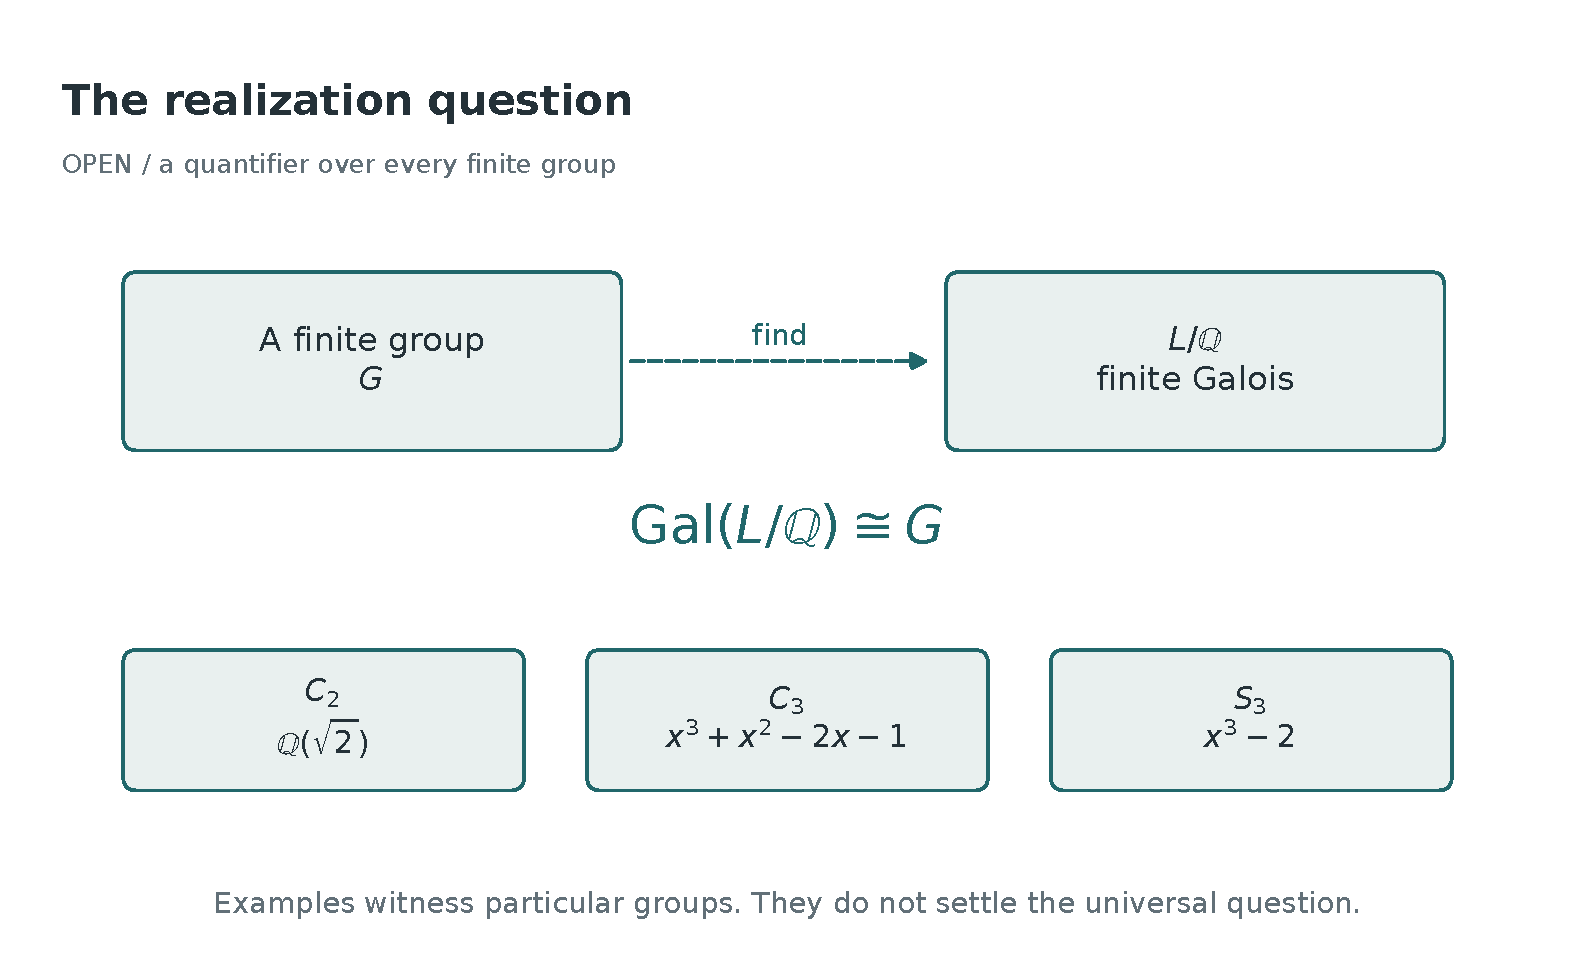
\includegraphics[width=0.96\linewidth]{../visual/figures/01_goal.pdf}
\caption{The inverse problem starts with a prescribed finite group and requires a finite Galois field extension over the fixed ground field $\Q$. A representation of the group supplies symmetry data. Arithmetic realization must additionally supply the field and its full automorphism group.}
\label{fig:g01-goal}
\end{figure}

\section{Why the splitting field is the relevant object}

Let $f\in\Q[X]$ be a nonconstant polynomial. A splitting field is a smallest field extension in which $f$ is a product of linear factors. It is unique up to an isomorphism that fixes $\Q$. In characteristic zero, every irreducible polynomial is separable. The splitting field of $f$ is therefore a finite Galois extension, even if $f$ itself is reducible or has repeated factors. Replacing $f$ by the product of its distinct irreducible factors does not change this field.

If $\alpha$ is just one root, the field $\Q(\alpha)$ can be smaller than the splitting field. The remaining roots need not lie in it. The equation $X^3-2=0$ will give our first explicit example of this distinction. Its real root generates a field of degree three, whereas the field containing all three roots has degree six.

\begin{proposition}[An equivalent polynomial formulation]
\label{prop:g01-polynomial}
Conjecture~\ref{conj:g01-igp} is equivalent to the following assertion. Every finite group is the Galois group of the splitting field over $\Q$ of some separable polynomial in $\Q[X]$.
\end{proposition}

\begin{proof}
A splitting field in characteristic zero is finite Galois, so the polynomial assertion gives the field assertion. Conversely, let $L/\Q$ be finite Galois. The primitive element theorem gives $L=\Q(\alpha)$ for some $\alpha$. Its minimal polynomial is separable. Normality says that every conjugate of $\alpha$ over $\Q$ belongs to $L$. Thus $L$ contains the splitting field. The splitting field also contains $\alpha$ and hence all of $L$, so the two fields agree. The primitive element theorem used here is a classical input for finite separable extensions \cite{Milne2022}.
\end{proof}

An integral polynomial can be used if desired. Clear denominators to obtain a polynomial in $\Z[X]$ with the same roots. The resulting polynomial need not be monic. Alternatively, multiply a primitive element by an integer large enough to make it integral and use its monic minimal polynomial. These changes concern presentation. They do not replace the requirement that the splitting field have the correct group.

\section{The action on roots}

Suppose $f$ has $d$ distinct roots in its splitting field $L$. Every automorphism of $L/\Q$ permutes them. The action is faithful because the roots generate $L$: an automorphism fixing every root fixes every rational expression in those roots. Consequently
\begin{equation}
\label{eq:g01-root-action}
\Gal(L/\Q)\hookrightarrow S_d.
\end{equation}
If $f$ is irreducible, the action is transitive. One way to see this is to send any root to any other through the isomorphism between the corresponding simple extensions, then extend that embedding to the splitting field. Normality ensures that the resulting embedding is an automorphism of $L$. This standard extension theorem is included in the finite Galois framework \cite{Milne2022}.

Transitivity does useful work. The orbit of a root has size $d$, so the order of the group is divisible by $d$. It does not identify the group by itself. A cubic can have group $C_3$ or $S_3$. A quartic can have several transitive subgroups of $S_4$. The examples in the next chapter show how extra information selects the group.

\begin{figure}[tbp]
\centering
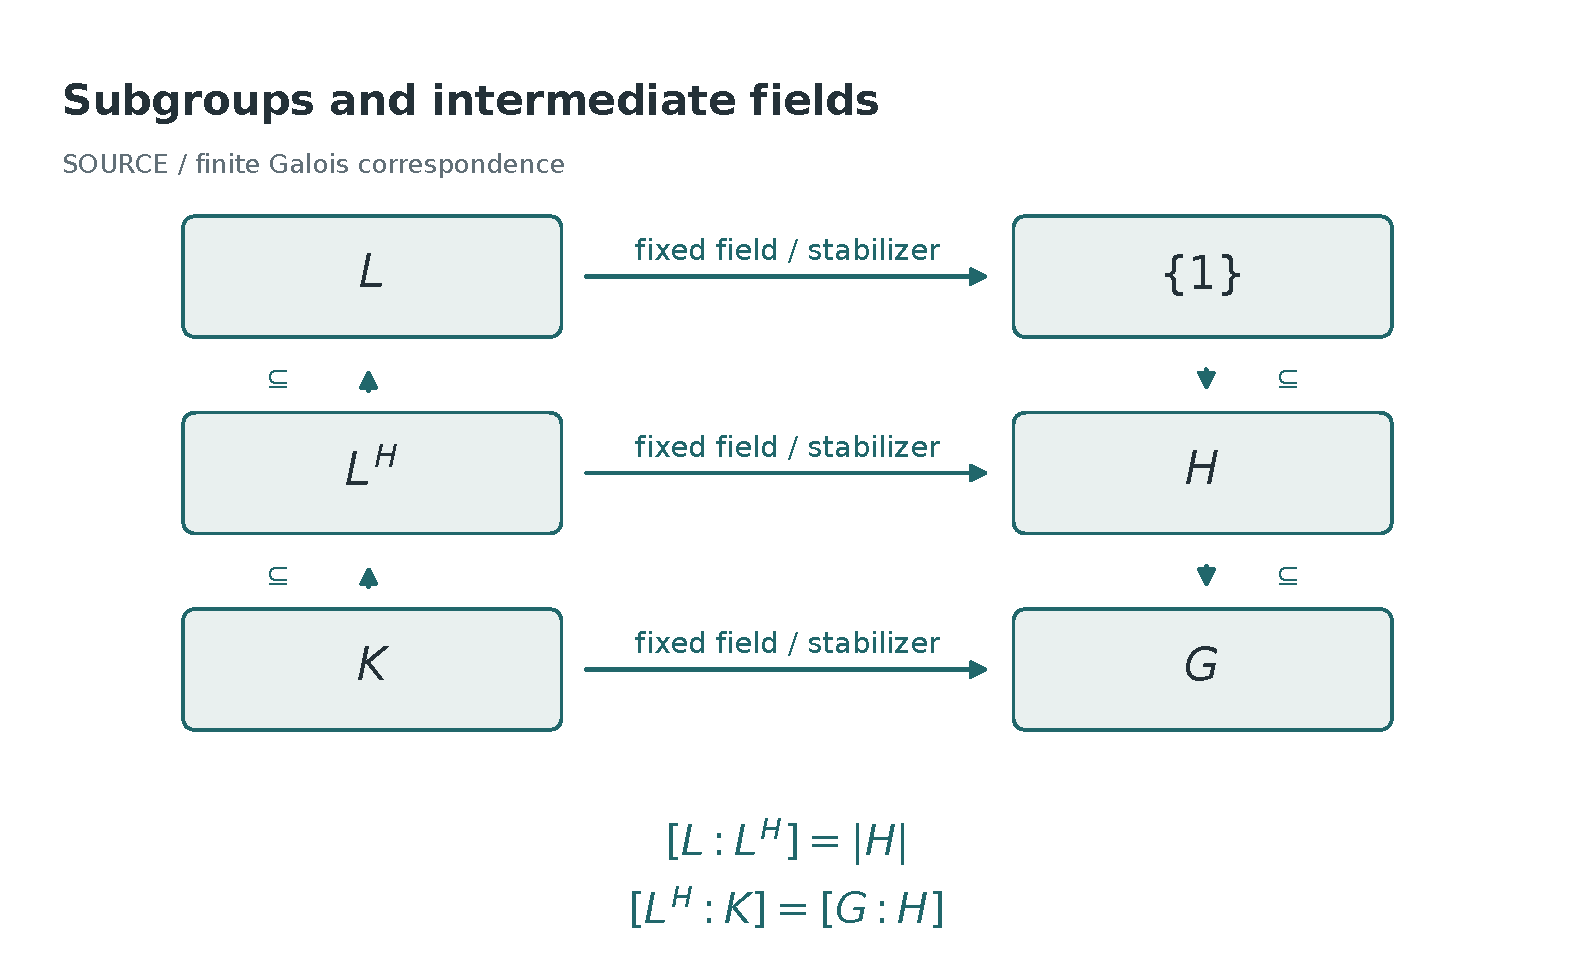
\includegraphics[width=0.96\linewidth]{../visual/figures/02_field_group.pdf}
\caption{For an already supplied finite Galois extension $L/K$ with group $G$, subgroups $H\le G$ correspond to intermediate fixed fields $L^H$. The direction of inclusion reverses. The classical correspondence computes degrees and organizes fields after the ambient field extension has been established \cite[Theorem 3.17]{Milne2022}.}
\label{fig:g01-field-group}
\end{figure}

\section{The regular representation supplies a model}

Let $G$ be any finite group. Its left regular action is the permutation action on its own underlying set,
\[
g\cdot h=gh.
\]
It is faithful: if $g$ fixes the identity element, then $g=1$. On the vector space $\Q^G$ with basis $e_h$, the corresponding operators are
\[
\rho(g)e_h=e_{gh}.
\]
They satisfy $\rho(g_1g_2)=\rho(g_1)\rho(g_2)$ and give an embedding $G\hookrightarrow\operatorname{GL}(\Q^G)$. These are exact constructions for every finite group.

They do not yet give an extension of $\Q$. The vector space $\Q^G$ has no designated field multiplication. Its coordinatewise multiplication makes it a product algebra, which has zero divisors whenever $|G|>1$. For distinct $h,k$, the coordinate idempotents satisfy $e_he_k=0$ although both are nonzero. A finite product of copies of $\Q$ is a useful algebraic symmetry model, but it cannot be the required nontrivial number field.

A proposed rational bilinear multiplication would only begin the next test. It must be commutative and associative, have a unit and have no zero divisors. In finite dimension these properties make it a field: multiplication by a nonzero element is an injective linear map and hence is surjective, so the element has an inverse. The action must also preserve that multiplication. Then one must prove that the fixed field is $\Q$ and that the full automorphism group is the chosen $G$. The finite automorphism theorem can discharge the last group calculation once an actual field and actual field automorphisms are available. It does not manufacture those inputs.

\begin{claimboundary}
Faithful permutation and matrix realizations exist for every finite group. They prove that finite symmetry can be represented exactly. The inverse Galois conjecture asks whether that symmetry can always be realized as the full automorphism group of a finite field extension of $\Q$.
\end{claimboundary}

This distinction will remain central when projector packets and transfer operators enter the discussion. Such structures can preserve information about a group action or about an extension already supplied. They have to carry additional arithmetic construction data before they can prove that a new extension exists. The following examples supply genuine fields, not only representations.

\chapter{Five complete field realizations}
\label{chap:g02-examples}

\section{Quadratic symmetry: $C_2$}

Let $\alpha=\sqrt2$ and $L=\Q(\alpha)$. The polynomial $X^2-2$ is irreducible over $\Q$. Indeed, if $a/b$ in lowest terms had square two, then $a^2=2b^2$ would make $a$ even. Writing $a=2c$ gives $b^2=2c^2$, so $b$ would also be even, a contradiction.

Every element of $L$ has a unique expression $a+b\alpha$ with $a,b\in\Q$. The map
\[
\sigma(a+b\alpha)=a-b\alpha
\]
preserves addition and multiplication because both $\alpha$ and $-\alpha$ satisfy the same relation $\alpha^2=2$. It fixes $\Q$, has square the identity, and is nontrivial. The only possible images of $\alpha$ under a rational automorphism are $\alpha$ and $-\alpha$. Thus there are exactly two automorphisms.

The polynomial already splits in $L$, so $L/\Q$ is Galois and
\[
\Gal(L/\Q)=\{1,\sigma\}\simeq C_2.
\]
Its fixed elements satisfy $a+b\alpha=a-b\alpha$, whence $b=0$. This directly checks $L^{\langle\sigma\rangle}=\Q$ without appealing to an abstract correspondence. The same argument works for every nonsquare $d\in\Q^\times$, with $\sqrt2$ replaced by $\sqrt d$.

\section{Two independent signs: $V_4$}

Now take
\[
L=\Q(\sqrt2,\sqrt3).
\]
The second square root does not belong to $\Q(\sqrt2)$. If $\sqrt3=a+b\sqrt2$, squaring and comparing the rational and $\sqrt2$ parts gives $2ab=0$ and $a^2+2b^2=3$. If $b=0$, a rational square would be three. If $a=0$, a rational square would be $3/2$. Neither is possible, as the prime exponents in a rational square are even. Thus the tower has degrees two and two, and $[L:\Q]=4$.

The four elements
\[
1,\quad\sqrt2,\quad\sqrt3,\quad\sqrt6
\]
form a rational basis. Independent choices of signs define four automorphisms. Let $s$ change the sign of $\sqrt2$ and let $t$ change the sign of $\sqrt3$. They satisfy
\[
s^2=t^2=1,\qquad st=ts.
\]
They are distinct because their effects on the two generators are distinct. The extension is the splitting field of $(X^2-2)(X^2-3)$, so it is Galois. Since the degree is four, these four automorphisms are the full group:
\[
\Gal(L/\Q)\simeq C_2\times C_2=V_4.
\]

\begin{figure}[tbp]
\centering
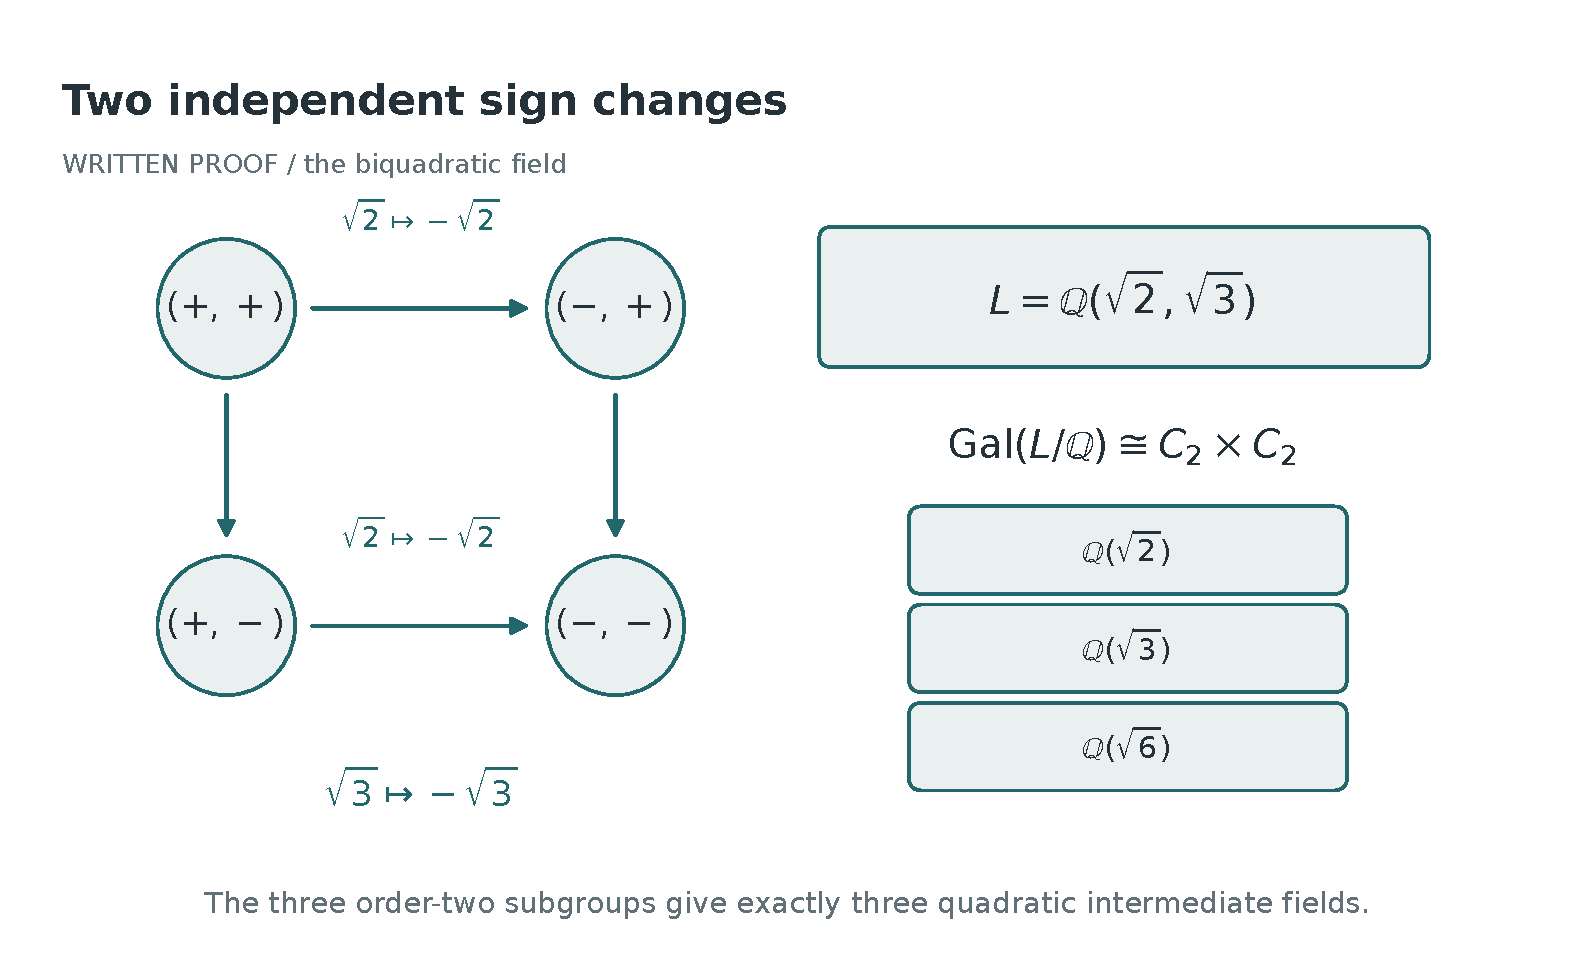
\includegraphics[width=0.96\linewidth]{../visual/figures/04_biquadratic.pdf}
\caption{The biquadratic field has three quadratic intermediate fields. Their sign symmetries give the three subgroups of order two in $V_4$. The degree calculations and fixed elements are proved directly in the text.}
\label{fig:g02-biquadratic}
\end{figure}

The fixed fields can also be read directly from the basis. The elements fixed by $s$ are $a+c\sqrt3$, so $L^{\langle s\rangle}=\Q(\sqrt3)$. Similarly, $L^{\langle t\rangle}=\Q(\sqrt2)$. The product $st$ changes the signs of both square roots but fixes their product, giving $L^{\langle st\rangle}=\Q(\sqrt6)$. An element fixed by both $s$ and $t$ has only its rational component left.

This example already exhibits a later theme. Averaging the operators $1$ and $s$ keeps the $1$ and $\sqrt3$ components while removing the other two. That operation recognizes a fixed subspace in a field already constructed. The proof that this subspace is the quadratic field $\Q(\sqrt3)$ uses the multiplication inherited from $L$.

\section{A cyclic cubic with discriminant $49$}

Consider
\[
f(X)=X^3+X^2-2X-1.
\]
The rational root theorem restricts rational roots to $1$ and $-1$. Since $f(1)=-1$ and $f(-1)=1$, there is no rational root. A reducible cubic over a field has a linear factor, so $f$ is irreducible.

For a monic cubic $X^3+aX^2+bX+c$, the discriminant is
\[
a^2b^2-4b^3-4a^3c-27c^2+18abc.
\]
Here this gives
\begin{equation}
\label{eq:g02-cubic-disc}
\operatorname{disc}(f)=4+32+4-27+36=49.
\end{equation}
The discriminant is nonzero, so the roots are distinct.

We can see the splitting field without using the discriminant criterion. Let $\alpha$ be a root. In $\Q(\alpha)$, the defining equation gives
\[
\alpha^3=-\alpha^2+2\alpha+1,
\qquad
\alpha^4=3\alpha^2-\alpha-1.
\]
Set
\[
\beta=\alpha^2-2,
\qquad
\gamma=-\alpha^2-\alpha+1.
\]
Direct reduction by the two displayed identities gives
\begin{equation}
\label{eq:g02-three-roots}
\alpha+\beta+\gamma=-1,
\quad
\alpha\beta+\alpha\gamma+\beta\gamma=-2,
\quad
\alpha\beta\gamma=1.
\end{equation}
Thus
\[
f(X)=(X-\alpha)(X-\beta)(X-\gamma)
\quad\text{in }\Q(\alpha)[X].
\]
For example, the second identity follows from
\[
\alpha(\beta+\gamma)=-\alpha-\alpha^2,
\qquad
\beta\gamma=\alpha^2+\alpha-2.
\]
The third follows by multiplying the latter expression by $\alpha$ and using the cubic relation. These are exact algebraic equalities, not numerical root approximations.

Since $f$ is irreducible, $[\Q(\alpha):\Q]=3$. Since it splits there, the root field is already its splitting field. Its Galois group has order three and is therefore cyclic. There is an explicit generator sending $\alpha$ to $\beta$. The map is well defined because $\beta$ is another root of the same irreducible polynomial. It is a field embedding into $\Q(\alpha)$ and hence an automorphism, since the image has degree three. The identities
\[
\beta^2-2=\gamma,
\qquad
\gamma^2-2=\alpha
\]
show that this automorphism cycles the three roots. Their distinctness also follows from the nonzero discriminant.

\begin{figure}[tbp]
\centering
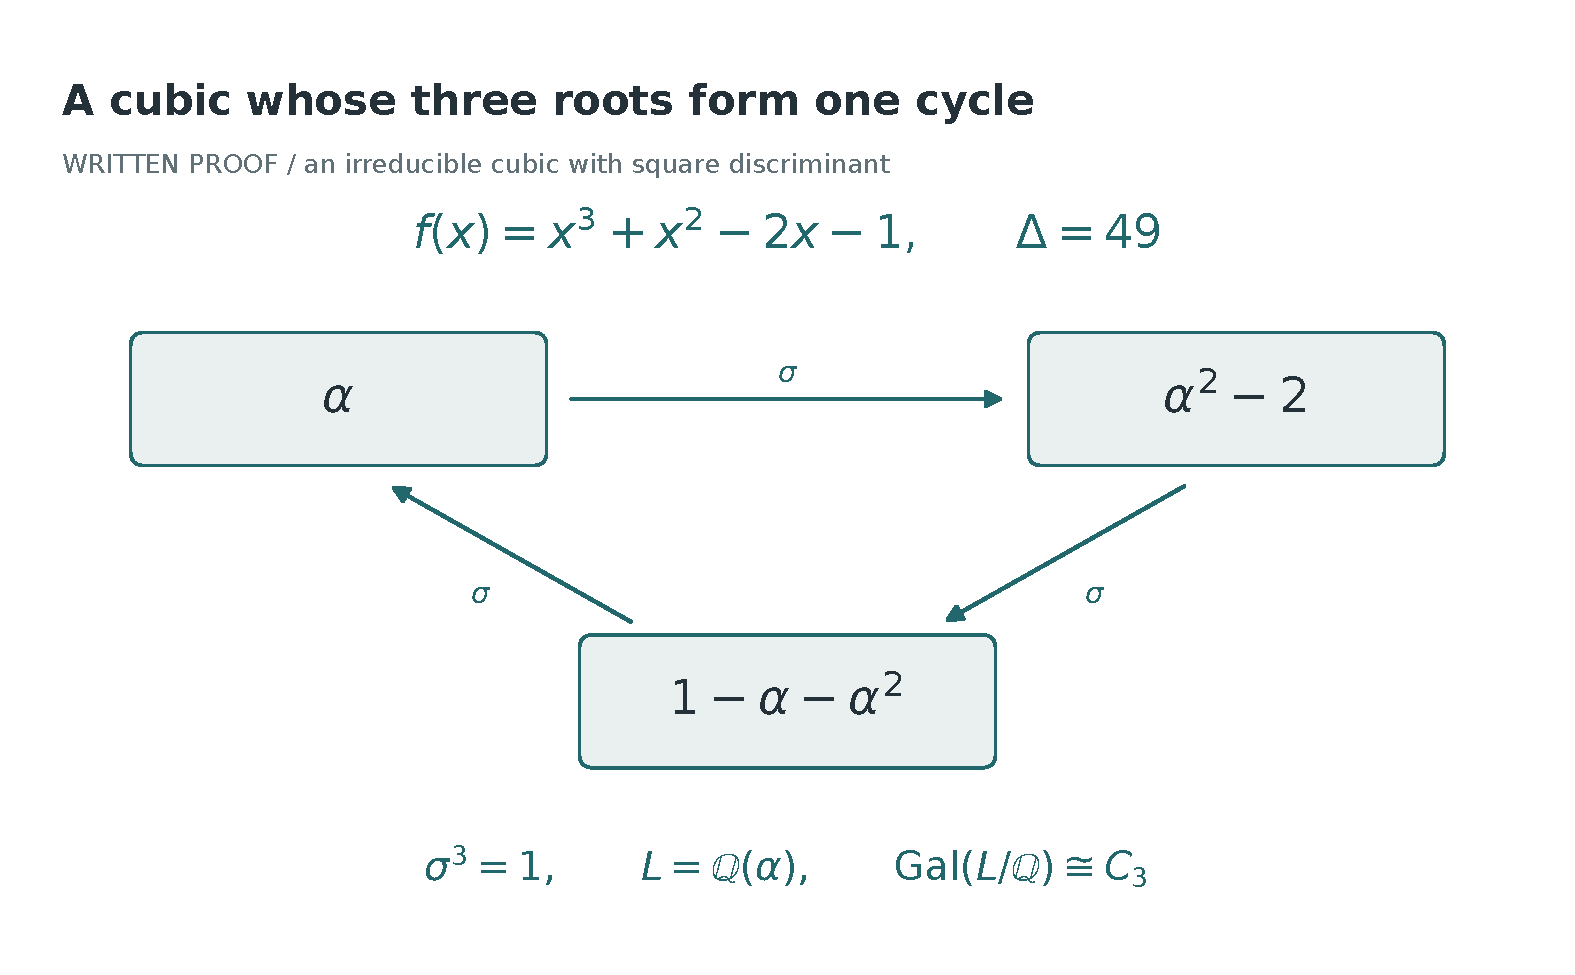
\includegraphics[width=0.96\linewidth]{../visual/figures/05_cyclic_cubic.pdf}
\caption{The cubic realization closes inside one root field. The transformation $r\mapsto r^2-2$ cycles its three roots, and their exact symmetric identities recover the original polynomial. The group has order three because the polynomial is irreducible and already splits in that field.}
\label{fig:g02-cyclic-cubic}
\end{figure}

The discriminant offers a second group check. If $r_1,r_2,r_3$ are the roots, the Vandermonde product $V=\prod_{i<j}(r_i-r_j)$ satisfies $V^2=49$. In a field of characteristic zero, this implies $V=7$ or $V=-7$, so every rational automorphism fixes $V$. Permuting the roots multiplies $V$ by the sign of the permutation. The group is therefore contained in $A_3$. Irreducibility makes it transitive, forcing it to be $A_3\simeq C_3$. This is a useful cross check of the explicit field computation. The figure labels the discriminant itself by $\Delta$, so $V^2=\Delta$.

\section{A cubic whose root field is too small: $S_3$}

Take $f(X)=X^3-2$ and let $\alpha$ denote its positive real root. Eisenstein's criterion at the prime two proves that $f$ is irreducible. Equivalently, a rational root would have to be an integer divisor of two, and none has cube two. Let $\zeta$ be a primitive cube root of unity, so
\[
\zeta^2+\zeta+1=0.
\]
The three roots are $\alpha,\zeta\alpha,\zeta^2\alpha$. Their splitting field is
\[
L=\Q(\alpha,\zeta).
\]
Indeed, this field contains every root, and the ratio of the second root to the first recovers $\zeta$ from the splitting field.

The field $\Q(\alpha)$ is contained in $\R$, whereas $\zeta$ is nonreal. Thus $\zeta\notin\Q(\alpha)$. Its quadratic equation remains irreducible over this real field, and
\begin{equation}
\label{eq:g02-s3-degree}
[L:\Q]=[L:\Q(\alpha)]\,[\Q(\alpha):\Q]=2\cdot3=6.
\end{equation}
The faithful action on three roots embeds $\Gal(L/\Q)$ into $S_3$. Both groups have order six, so the embedding is an isomorphism.

There is also a concrete pair of generators. Over $\Q(\zeta)$, the element $\alpha$ has degree three: the tower degree is $[L:\Q(\zeta)]=3$. Sending $\alpha$ to $\zeta\alpha$ while fixing $\zeta$ therefore gives an automorphism $\tau$ of order three. Complex conjugation gives an automorphism $c$ of order two that fixes $\alpha$ and sends $\zeta$ to $\zeta^2$. On the generators,
\[
c\tau c=\tau^{-1}.
\]
Hence the cyclic cubic subgroup is inverted by the other generator, as in the usual presentation of $S_3$.

The discriminant is $-108$. In particular it is not a square in $\Q$, agreeing with the presence of odd permutations. The degree calculation is already a complete proof, so the discriminant is corroborating information rather than an extra hypothesis. This separation prevents the example from becoming dependent on every possible way of recognizing its group.

\section{A quartic with cycle certificates: $S_4$}

For a quartic realization, consider
\[
f(X)=X^4-X-1.
\]
Its reduction modulo two is $X^4+X+1$. It has no root in $\mathbf F_2$. The only monic irreducible quadratic over $\mathbf F_2$ is $X^2+X+1$. Modulo that polynomial, $X^2=X+1$, $X^3=1$ and $X^4=X$, so $X^4+X+1$ has remainder one. A reducible quartic without a linear factor must factor as two irreducible quadratics. This possibility has just been excluded, proving that the reduction is irreducible. Gauss's lemma now proves that $f$ is irreducible over $\Q$.

We use one classical bridge between modular factorization and a characteristic zero group.

\begin{theorem}[Good prime cycle theorem, external input]
\label{thm:g02-cycle}
Let $f\in\Z[X]$ be monic, and suppose its reduction modulo a prime $p$ is squarefree. If its irreducible factors over $\mathbf F_p$ have degrees $d_1,\ldots,d_r$, the Galois group of its splitting field over $\Q$, acting on the roots of $f$, contains a permutation with disjoint cycle lengths $d_1,\ldots,d_r$.
\end{theorem}

This is the Frobenius factorization theorem in the stated squarefree setting \cite[Theorem 4.28]{Milne2022}. The theorem is external. The polynomial identities and the following finite irreducibility checks are displayed explicitly, so their role does not depend on trusting a numerical group label returned by software.

Modulo two, irreducibility gives a four cycle. Squarefreeness holds since the derivative of $X^4+X+1$ is one. Modulo seven there is the exact factorization
\begin{equation}
\label{eq:g02-mod-seven}
f(X)=(X-3)(X^3+3X^2+2X+5)
\quad\text{in }\mathbf F_7[X].
\end{equation}
The cubic takes the following values:
\[
\begin{array}{c|rrrrrrr}
x&0&1&2&3&4&5&6\\\hline
x^3+3x^2+2x+5\pmod7&5&4&1&2&6&5&5.
\end{array}
\]
It has no root, hence is irreducible. Its derivative $3X^2+6X+2$ is nonzero and has smaller degree, so it cannot have a common factor with this irreducible cubic. The cubic's value at three is two, so the linear factor is distinct. The reduction is squarefree. The cycle theorem therefore gives a permutation with one fixed point and one three cycle.

\begin{figure}[tbp]
\centering
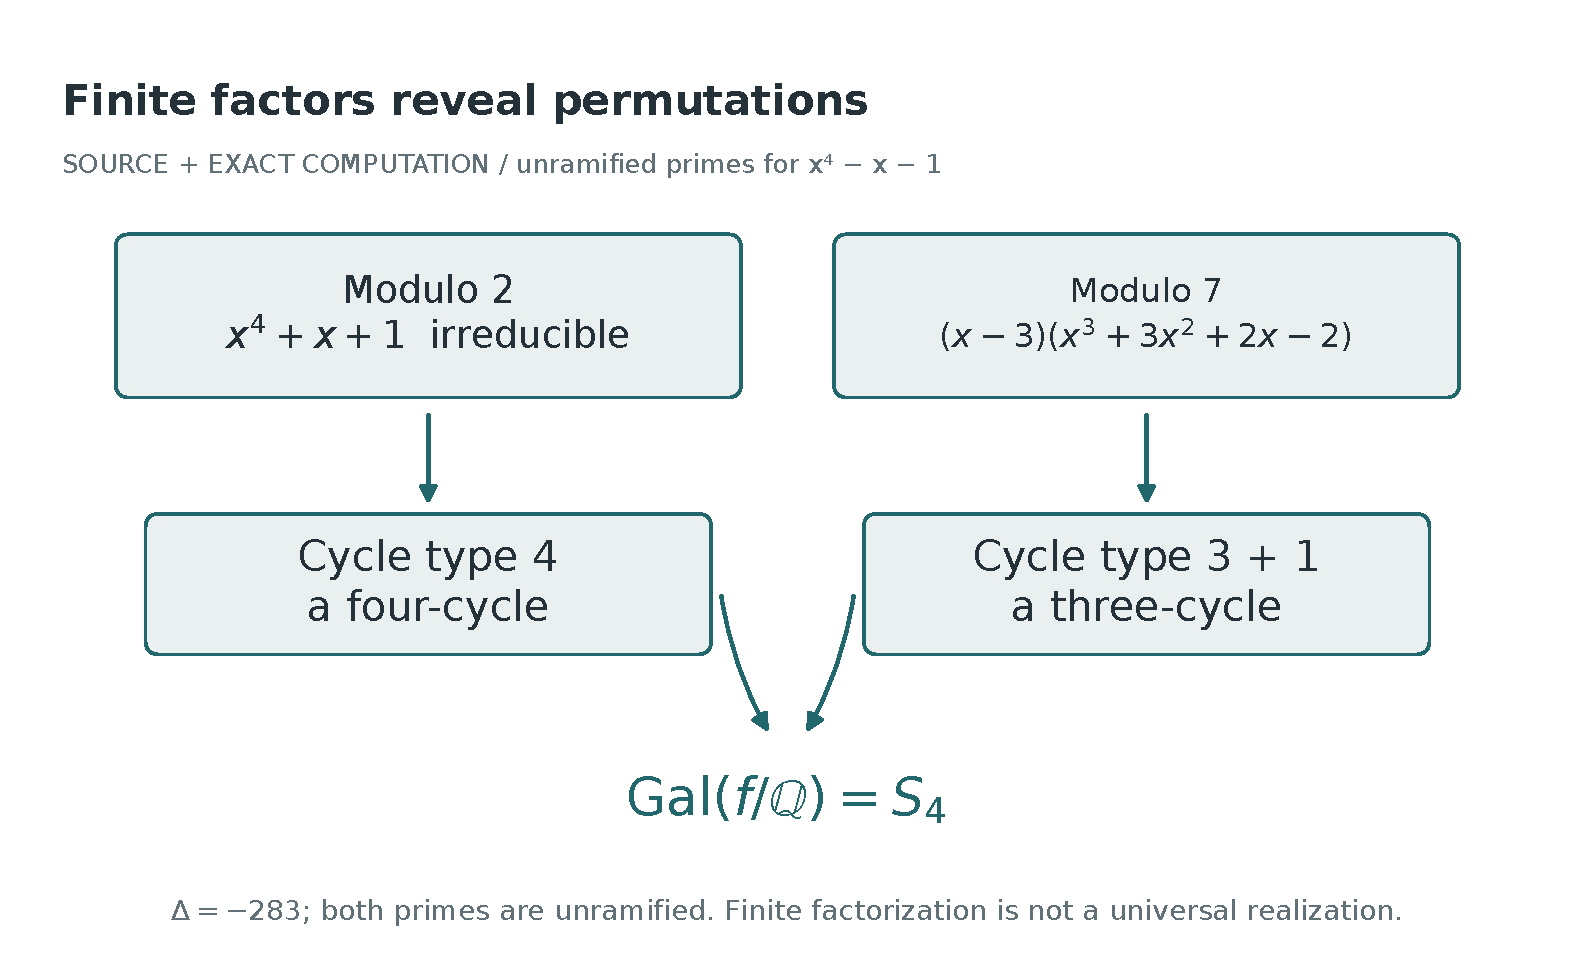
\includegraphics[width=0.96\linewidth]{../visual/figures/07_factor_cycle.pdf}
\caption{The modular certificates for $X^4-X-1$ produce a four cycle at two and a three cycle at seven. Squarefreeness is checked at both primes. A short subgroup argument then identifies the characteristic zero group as $S_4$. These two exact prime calculations certify this polynomial, not a family of arbitrary groups.}
\label{fig:g02-factor-cycle}
\end{figure}

Let $H$ be the Galois group in its faithful action on four roots. Its order is divisible by four and three, so it is divisible by twelve. Since $H\le S_4$, its order is twelve or twenty four. A subgroup of order twelve would have index two and would be normal. The quotient map $S_4\to C_2$ would send all transpositions to the same element because they are conjugate. They generate $S_4$, so this element must be nontrivial. Its kernel is therefore exactly $A_4$, the permutations expressible as a product of an even number of transpositions. But a four cycle is odd. Since $H$ contains one, $H$ cannot be $A_4$. It follows that $H=S_4$.

\begin{resultbox}
The fields above realize $C_2$, $V_4$, $C_3$, $S_3$ and $S_4$ over $\Q$. Each conclusion has a finite, complete proof. The quartic proof imports the good prime cycle theorem and combines it with explicit factorization checks and a proved subgroup argument.
\end{resultbox}

These examples answer five individual existence questions. Their value is not a numerical extrapolation to all finite groups. They make the required ingredients visible: an actual field, controlled degree, full root closure and enough information to identify the entire group. A general construction has to furnish counterparts of those ingredients for an arbitrary prescribed $G$.

\chapter{Every group acts on a field, but the base changes}
\label{chap:g03-generic}

\section{Independent variables keep the action faithful}

Fix a finite group $G$. For every $g\in G$, introduce an independent variable $x_g$. Let
\[
E=\Q(x_g\mid g\in G)
\]
be the rational function field in these $|G|$ variables. Algebraic independence means that no nonzero polynomial with rational coefficients in the $x_g$ vanishes. In particular distinct variables are distinct elements of $E$.

For $h\in G$, define
\begin{equation}
\label{eq:g03-variable-action}
\sigma_h(x_g)=x_{hg},\qquad\sigma_h(q)=q\quad(q\in\Q).
\end{equation}
A permutation of independent variables extends to an automorphism of the polynomial ring and then of its fraction field. The inverse is $\sigma_{h^{-1}}$. The action satisfies $\sigma_h\sigma_k=\sigma_{hk}$, so it is a group action by genuine field automorphisms. It is faithful because $\sigma_h(x_1)=x_h$ differs from $x_1$ when $h\ne1$.

Let
\[
K=E^G=\{z\in E:\sigma_h(z)=z\text{ for every }h\in G\}.
\]
This is a field containing $\Q$. Unlike the vector space model in Chapter~\ref{chap:g01-question}, we now have field multiplication and a faithful action preserving it. The finite automorphism theorem can therefore be applied with its actual hypotheses satisfied.

\begin{figure}[tbp]
\centering
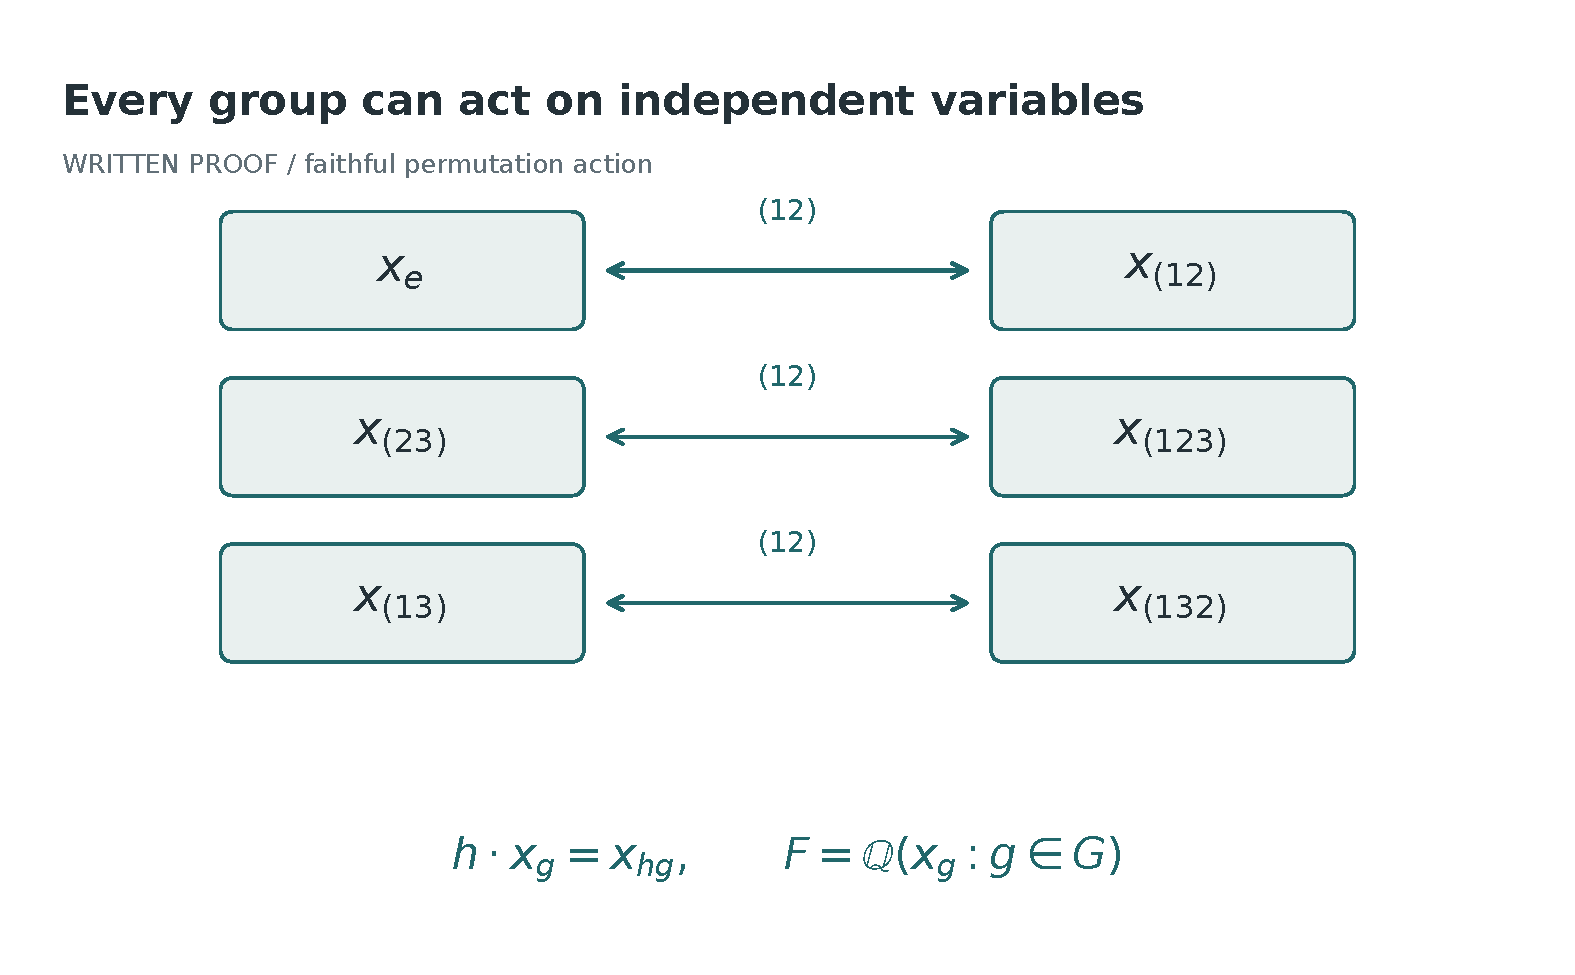
\includegraphics[width=0.96\linewidth]{../visual/figures/08_generic_variables.pdf}
\caption{Independent variables turn the left regular permutation action into an action by field automorphisms. The diagram illustrates multiplication by $(12)$ in $S_3$ and writes $F$ for the field called $E$ in the text, with $e=1$ for the group identity. Artin's theorem realizes the group over its fixed field $K$, while the required arithmetic base remains $\Q$.}
\label{fig:g03-variables}
\end{figure}

\section{The fixed field theorem and its exact conclusion}

\begin{theorem}[Artin's finite automorphism theorem, external input]
\label{thm:g03-artin}
Let $E$ be a field and $A$ a finite subgroup of $\Aut(E)$. If $K=E^A$, then $E/K$ is a finite Galois extension,
\[
[E:K]=|A|,
\qquad
\Gal(E/K)=A.
\]
\end{theorem}

The theorem, with no finiteness assumption on $E$ over some preassigned smaller field, is the classical finite automorphism theorem \cite[Corollary 3.11]{Milne2022}. Its important finiteness condition is on the acting subgroup $A$. It is not a theorem about an arbitrary infinite group of automorphisms.

Applied to~\eqref{eq:g03-variable-action}, it gives
\begin{equation}
\label{eq:g03-generic-extension}
\Gal(E/K)\simeq G,
\qquad
[E:K]=|G|.
\end{equation}
This is a universal realization over a group dependent field $K$. It proves that no finite abstract group is incompatible with field automorphism structure. It leaves the chosen arithmetic base untouched.

An orbit polynomial gives a useful piece of the theorem's mechanism. For any $a\in E$,
\[
P_a(T)=\prod_{h\in G}(T-\sigma_h(a))
\]
has coefficients in $K$, since the action permutes its factors. Thus every element of $E$ is algebraic over $K$. Orbit repetitions are allowed, so this polynomial need not be the minimal polynomial and can have repeated factors. The fact that all such elements together generate a finite extension of degree exactly $|G|$ is the content of Artin's theorem. Bounded degrees for individual elements should not be substituted for that theorem without a further argument.

In our particular construction, $a=x_1$ has $|G|$ distinct images. The polynomial
\begin{equation}
\label{eq:g03-orbit-polynomial}
P(T)=\prod_{g\in G}(T-x_g)
\end{equation}
has degree $|G|$ and coefficients in $K$. Any polynomial over $K$ vanishing at $x_1$ vanishes at every $x_g$ after applying the automorphisms. It therefore has at least $|G|$ distinct roots. The minimal polynomial of $x_1$ has degree $|G|$. In view of~\eqref{eq:g03-generic-extension},
\[
E=K(x_1).
\]
This establishes a primitive element explicitly for the generic extension. The labels on its roots still encode the regular action.

\section{Why the invariant base is not $\Q$}

Already the invariant
\[
s=\sum_{g\in G}x_g
\]
is transcendental over $\Q$. If a nonzero polynomial $F\in\Q[T]$ satisfied $F(s)=0$, then $F(\sum_gx_g)$ would be a zero polynomial in independent variables. Substituting zero for every variable except $x_1$ would give the impossible identity $F(x_1)=0$. Thus $s\in K\setminus\Q$.

More generally, $E/K$ is algebraic, so the two fields have the same transcendence degree over $\Q$:
\begin{equation}
\label{eq:g03-transdegree}
\operatorname{trdeg}_{\Q}K=\operatorname{trdeg}_{\Q}E=|G|.
\end{equation}
The finite degree $[E:K]$ does not make $E$ or $K$ finite over $\Q$. Both retain transcendental parameters. For the trivial group, the construction says only that $E=K=\Q(x_1)$, whereas its arithmetic realization was simply $\Q$. Even this endpoint shows why changing the base cannot be silently ignored.

There is another issue. Knowing the transcendence degree of $K$ does not prove that $K$ is a rational function field. A field of transcendence degree $d$ can be a nontrivial algebraic extension of $\Q(t_1,\ldots,t_d)$. The assertion that a particular invariant field is purely transcendental is a separate rationality problem, commonly called Noether's problem for this action. It must be supplied or proved for the group under consideration. Milne reports Swan's counterexample to universal rationality for the usual permutation action \cite[Aside 5.41]{Milne2022}. We have not independently audited Swan's original counterexample. This is source attributed context and is not a dependency of the conditional realization argument below. Failure of rationality for a group would not rule out a different inverse Galois construction.

\begin{figure}[tbp]
\centering
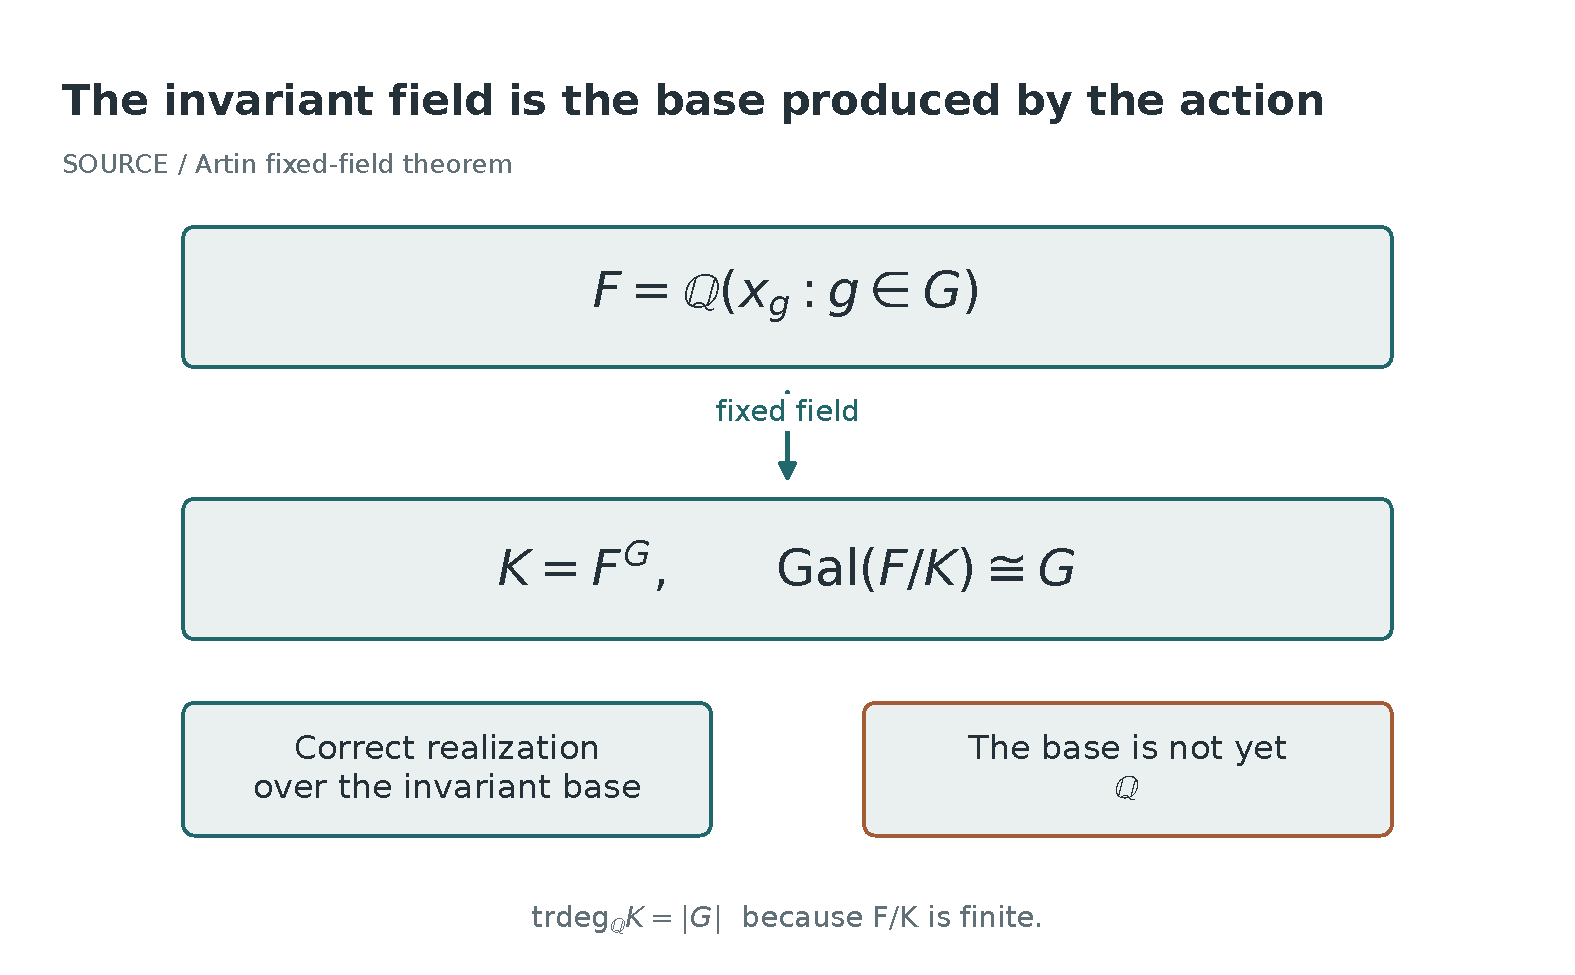
\includegraphics[width=0.96\linewidth]{../visual/figures/09_invariant_base.pdf}
\caption{The invariant field contains rational constants and also transcendental invariants. The diagram writes $F=E$ and $K=F^G$. Its transcendence degree is fixed by the finite extension $E/K$. Pure transcendence requires an additional rationality argument before Hilbert specialization can be applied through a rational parameter presentation.}
\label{fig:g03-invariant-base}
\end{figure}

\section{A sufficient rationality route}

\begin{definition}
An extension $E/\Q(t_1,\ldots,t_d)$ is regular over $\Q$ if every element of $E$ algebraic over $\Q$ belongs to $\Q$. In the characteristic zero setting considered here, this is the constant field condition used for regular finite Galois extensions.
\end{definition}

Our rational function field $E=\Q(x_g)$ has this property. To see the constant field assertion directly, suppose $r\in E$ is algebraic over $\Q$. Write $r=A/B$ for polynomials over $\Q$ with $B\ne0$. There is a rational tuple at which $B$ is nonzero: a nonzero polynomial over the infinite field $\Q$ cannot vanish on every rational tuple, by induction on the number of variables. A monic minimal polynomial $m\in\Q[T]$ satisfies $m(A/B)=0$ identically. Evaluating at that tuple gives a rational root of $m$. Irreducibility forces $m$ to have degree one, so $r\in\Q$.

\begin{theorem}[Hilbert specialization, external input]
\label{thm:g03-hilbert}
Let $d\ge1$ and let $E/\Q(t_1,\ldots,t_d)$ be a finite regular Galois extension with group $G$. There is a Hilbert subset of rational parameter tuples for which specialization is defined and the specialized extension has full Galois group $G$. The tuples may be required to avoid the zero set of any prescribed nonzero polynomial that records finitely many excluded denominators or discriminants.
\end{theorem}

This form combines the specialization theorem with Hilbert irreducibility and its Zariski density statement for rational Hilbert subsets \cite[Theorem 2.6.3, Theorem 5.2.4 and Proposition 5.2.14]{DebesLectureNotes}. It is an imported arithmetic theorem. The phrase ``full group'' is substantive. Outside an exceptional algebraic locus, a specialization can still have a proper subgroup. Hilbert irreducibility provides parameters retaining the needed irreducibility and hence the full degree, not merely parameters at which a polynomial remains defined.

\begin{proposition}[Rational invariant field is sufficient]
\label{prop:g03-noether-route}
For the regular variable action above, suppose the invariant field has a rational presentation
\[
K=\Q(t_1,\ldots,t_d)
\]
with algebraically independent $t_1,\ldots,t_d$. Then $G$ occurs as a Galois group over $\Q$.
\end{proposition}

\begin{proof}
By~\eqref{eq:g03-transdegree}, $d=|G|$, so $d\ge1$. Artin's theorem gives a finite Galois extension $E/K$ with group $G$. The preceding constant field argument proves that $E$ is regular over $\Q$. With the assumed presentation of $K$, all hypotheses of Theorem~\ref{thm:g03-hilbert} hold. A full group specialization gives a finite Galois extension of $\Q$ with group $G$.
\end{proof}

The proposition is a sufficient implication. It does not say that every realization over $\Q$ must come from this particular invariant field or that inverse Galois and Noether rationality are equivalent. A different regular construction, or a direct number field construction, may realize a group without resolving this invariant field's rationality. The proof also does not specify effective parameter sizes. An existence theorem for a Hilbert subset is different from a complete practical search algorithm with a prescribed stopping bound.

\section{Specialization can lose symmetry}

The smallest example makes the warning exact. Let $G=C_2$ exchange two variables $x,y$. Define
\[
s=x+y,\qquad p=xy.
\]
The variables $x,y$ are the roots of $T^2-sT+p$. Since $y=s-x$, the field $\Q(x,y)$ has degree at most two over $\Q(s,p)$. The nontrivial exchange fixes $s,p$, and $x\notin\Q(s,p)$ because an element in that field would be fixed. Hence the degree is exactly two. Artin's theorem then shows
\[
\Q(x,y)^{C_2}=\Q(s,p).
\]
The parameters $s,p$ are algebraically independent: the algebraic extension to $\Q(x,y)$ preserves transcendence degree two.

At $(s,p)=(0,-2)$ the polynomial becomes $T^2-2$, giving the quadratic realization already proved. At $(s,p)=(0,-1)$ it becomes $T^2-1$ and splits over $\Q$, so its splitting field has trivial group. Both discriminants are nonzero, respectively eight and four. Avoiding collisions alone therefore does not preserve the group. At $(s,p)=(2,1)$ the polynomial is $(T-1)^2$, which also fails separability. This is why a full group Hilbert specialization requires more than a nonzero discriminant.

\begin{openproblem}
For an arbitrary finite group, the variable action constructs a Galois extension over its invariant field. To turn this route into a realization over $\Q$, one must provide a suitable rational base presentation or another arithmetic construction. No claim that all invariant fields are rational is made here.
\end{openproblem}

The construction has isolated a genuine obligation. Symmetry is exact, the field is genuine, and the extension degree over the invariant base is known. What remains in this route is the passage to a suitable arithmetic base. The later chapters place that obligation beside the projector and packet language recovered from Operation Komorebi's earlier work.

\chapter{Subgroup symmetry as a resolved object}
\label{ch:subgroup-resolution}

The recovered Resolution Theory manuscript develops a direction that is both useful and exact. Once a finite group action has been supplied, subgroup invariants become ranges of averaging projectors. Inclusion, compatibility, and normality can then be read in an operator language. This chapter reconstructs that direction with proofs in the regular representation. The construction works for every finite group. Its input is the group, rather than a field over \(\Q\) having that group as its Galois group.

That distinction matters because the regular representation is available before any arithmetic realization has been found. It is a complete place to test the proposed subgroup calculus. An arithmetic extension, when one exists, can be translated into this language. Recovering the arithmetic extension from an arbitrary projector family requires more data, including multiplication and its descent to the desired base field.

\section{The regular module and its fixed ranges}

Let \(G\) be a finite group. Write \(V=\C[G]\) for the vector space with orthonormal basis \(\{\delta_g:g\in G\}\). The left regular action is
\begin{equation}
 \lambda(a)\delta_g=\delta_{ag}.
 \label{eq:b-regular-action}
\end{equation}
Every \(\lambda(a)\) is unitary. Extend \(\lambda\) linearly to the group algebra. This extension is injective, since
\begin{equation}
 \lambda\!\left(\sum_{g\in G}c_g g\right)\delta_1
 =\sum_{g\in G}c_g\delta_g.
 \label{eq:b-regular-faithfulness}
\end{equation}
Equality of regular operators therefore gives equality of all group algebra coefficients. This stronger property will justify the reverse implications below.

For \(H\leq G\), define
\begin{equation}
 e_H=\frac1{|H|}\sum_{h\in H}h\in\C[G],
 \qquad
 E_H=\lambda(e_H)=\frac1{|H|}\sum_{h\in H}\lambda(h).
 \label{eq:b-subgroup-average}
\end{equation}
The notation \(E_H\) in this chapter and its figures always means this operator. It is an average with normalization \(1/|H|\), rather than an unnormalized sum.

\begin{theorem}[Fixed range and rank]
\label{thm:b-fixed-range}
The operator \(E_H\) is the orthogonal projector onto
\[
 V^H=\{v\in V:\lambda(h)v=v\text{ for every }h\in H\}.
\]
Its rank is \([G:H]\). If \(H\leq K\), then
\begin{equation}
 E_HE_K=E_KE_H=E_K,
 \qquad V^K\subseteq V^H.
 \label{eq:b-nested-averages}
\end{equation}
\end{theorem}

\begin{proof}
Inversion permutes the elements of \(H\), so \(E_H^*=E_H\). Every element \(u\in H\) occurs exactly \(|H|\) times among the products \(hk\) with \(h,k\in H\). Consequently
\[
 E_H^2=\frac1{|H|^2}\sum_{h,k\in H}\lambda(hk)
 =\frac1{|H|}\sum_{u\in H}\lambda(u)=E_H.
\]
For \(a\in H\), left multiplication permutes the terms in the average, giving \(\lambda(a)E_H=E_H\). Thus its range consists of fixed vectors. Conversely, an \(H\) fixed vector is unchanged by every summand, and therefore by the average.

The orbits of \(H\) on the basis labels are the right cosets \(Hg\). For one representative \(g\) from each coset, put
\[
 v_{Hg}=|H|^{-1/2}\sum_{h\in H}\delta_{hg}.
\]
These vectors have disjoint supports, are orthonormal, and span the fixed range. Their number is \([G:H]\). Finally \(H\leq K\) makes every \(K\) fixed vector \(H\) fixed. Orthogonal projectors onto nested subspaces multiply to the projector onto the smaller subspace, in either order. This proves \eqref{eq:b-nested-averages}.
\end{proof}

In particular, the identity subgroup gives \(E_{\{1\}}=I\), while the whole group gives a rank one projector onto the constant vector. Every intermediate subgroup supplies a resolution \(\{E_H,I-E_H\}\). The word resolution here refers to the vector space decomposition into fixed vectors and their orthogonal complement. A field structure has not been imposed on these ranges.

The subgroup itself can be recovered from its regular average: the nonzero coefficients of \(E_H\delta_1\) have precisely the labels in \(H\). Thus distinct subgroups give distinct operators, including subgroups having the same order and the same projector rank. Rank by itself remembers the index, while the labelled operator remembers more.

\begin{figure}[tbp]
\centering
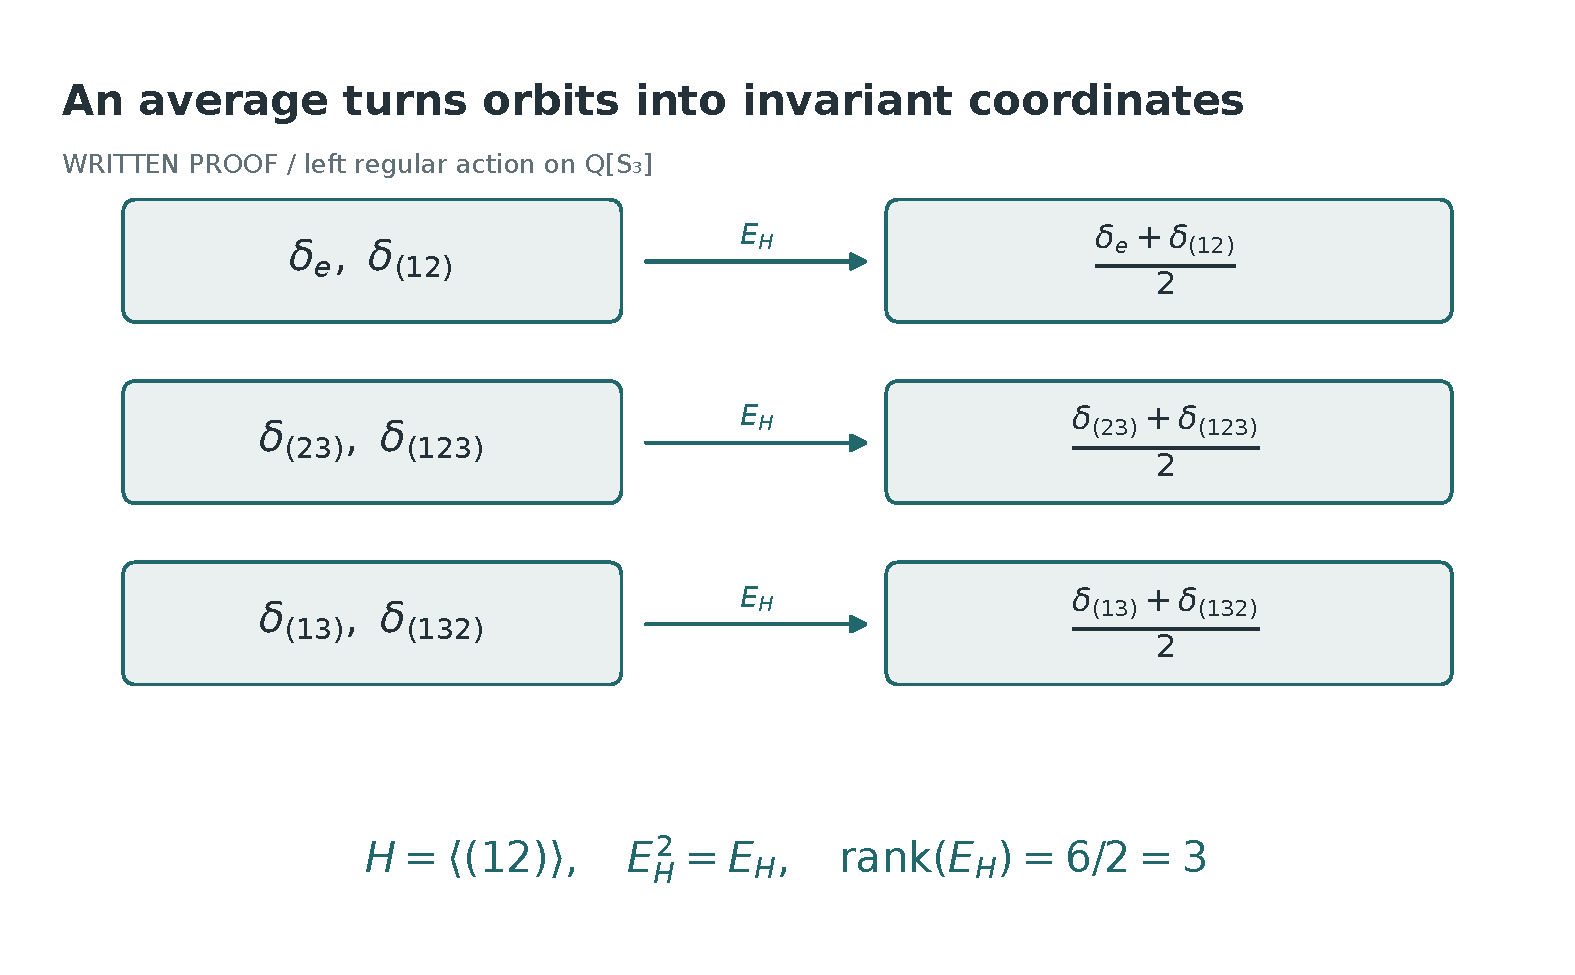
\includegraphics[width=0.96\linewidth]{../visual/figures/11_subgroup_projector.pdf}
\caption{The orbits of a subgroup's left action are the right cosets \(Hg\). Averaging replaces each orbit by one fixed vector, giving rank \([G:H]\). Enlarging the subgroup reduces the fixed range.}
\label{fig:b-subgroup-projector}
\end{figure}

\section{Products and the compatibility boundary}

For subgroups \(H,K\), the set \(HK=\{hk:h\in H,k\in K\}\) need not be a subgroup. The condition \(HK=KH\) is called permutability. It concerns the two product sets, and does not mean that every element of \(H\) commutes with every element of \(K\).

\begin{lemma}[Uniform product multiplicity]
\label{lem:b-product-multiplicity}
Every element of \(HK\) has exactly \(|H\cap K|\) expressions as \(hk\). Hence
\begin{equation}
 |HK|=\frac{|H||K|}{|H\cap K|},
 \qquad
 e_He_K=\frac1{|HK|}\sum_{x\in HK}x.
 \label{eq:b-product-support}
\end{equation}
The last sum is defined even when \(HK\) is not a subgroup.
\end{lemma}

\begin{proof}
Fix one expression \(x=h_0k_0\). An equality \(hk=h_0k_0\) is equivalent to \(h_0^{-1}h=k_0k^{-1}\in H\cap K\). For each \(a\in H\cap K\), the pair \((h_0a,a^{-1}k_0)\) gives one expression. This is a bijection. Counting all pairs proves the cardinality formula, and counting their coefficients in the group algebra proves the second identity.
\end{proof}

\begin{theorem}[Exact compatibility criterion]
\label{thm:b-compatible-averages}
In the regular realization, the following statements are equivalent:
\[
 HK=KH,\qquad HK\text{ is a subgroup},\qquad E_HE_K=E_KE_H.
\]
When they hold,
\begin{equation}
 E_HE_K=E_KE_H=E_{HK}=E_{\langle H,K\rangle}.
 \label{eq:b-compatible-product}
\end{equation}
Without a compatibility assumption, the intersection of the fixed ranges is still
\begin{equation}
 V^H\cap V^K=V^{\langle H,K\rangle}.
 \label{eq:b-fixed-intersection}
\end{equation}
\end{theorem}

\begin{proof}
If \(HK=KH\), then products of two elements of \(HK\) stay in \(HK\), because the middle factors can be written in the other order. Inversion sends \(HK\) to \(KH=HK\), and the identity belongs to it. It is therefore a subgroup. Conversely, if \(HK\) is a subgroup, its inverse set is itself, so \(KH=(HK)^{-1}=HK\).

For permutable subgroups, \eqref{eq:b-product-support} gives \(e_He_K=e_{HK}=e_Ke_H\). Applying \(\lambda\) proves the operator equality. If the operators commute, injectivity in \eqref{eq:b-regular-faithfulness} gives \(e_He_K=e_Ke_H\). Their supports are \(HK\) and \(KH\), with positive coefficients, so the sets are equal. A subgroup \(HK\) contains both \(H\) and \(K\), and is contained in every subgroup containing both, hence equals \(\langle H,K\rangle\). Finally, a vector fixed by both groups is fixed by every word in their elements and inverses. This proves the intersection identity without requiring their averages to commute.
\end{proof}

There is also an exact projector test. If \(P,Q\) are orthogonal projections and \(PQ\) is an orthogonal projection, then self adjointness gives \(PQ=(PQ)^*=QP\). In the compatible case, \(E_HE_K\) is the projection onto the common fixed range. In the incompatible case, one must retain the ordered products as transfers. Replacing them by a shared refinement would remove a real commutator.

\begin{example}[Two transpositions in \(S_3\)]
\label{ex:b-s3-incompatibility}
Let \(a=(12)\), \(b=(23)\), \(r=(123)\), and use permutation composition from right to left. Put \(H=\{1,a\}\), \(K=\{1,b\}\). Then \(ab=r\), \(ba=r^{-1}\), so
\[
 E_HE_K\delta_1=\tfrac14(\delta_1+\delta_a+\delta_b+\delta_r),
 \qquad
 E_KE_H\delta_1=\tfrac14(\delta_1+\delta_a+\delta_b+\delta_{r^{-1}}).
\]
In particular,
\begin{equation}
 [E_H,E_K]\delta_1
 =\tfrac14(\delta_r-\delta_{r^{-1}})\ne0.
 \label{eq:b-s3-commutator}
\end{equation}
Each average has rank three. Their common fixed range has rank one, because \(a,b\) generate \(S_3\). The rank one projector onto that intersection exists, even though it is not their ordered product.
\end{example}

For the figures we order the basis as
\[
 1,(12),(23),(13),(123),(132).
\]
The matrices of the two averages in this order are
\begin{equation}
 E_H=\frac12
 \begin{pmatrix}
 1&1&0&0&0&0\\
 1&1&0&0&0&0\\
 0&0&1&0&1&0\\
 0&0&0&1&0&1\\
 0&0&1&0&1&0\\
 0&0&0&1&0&1
 \end{pmatrix},
 \quad
 E_K=\frac12
 \begin{pmatrix}
 1&0&1&0&0&0\\
 0&1&0&0&0&1\\
 1&0&1&0&0&0\\
 0&0&0&1&1&0\\
 0&0&0&1&1&0\\
 0&1&0&0&0&1
 \end{pmatrix}.
 \label{eq:b-s3-matrices}
\end{equation}
The six columns of their commutator each have two entries of magnitude \(1/4\). Thus its squared Hilbert Schmidt norm is \(6\cdot2/16=3/4\). The exact computation bundle checks these matrices and all thirty six ordered pairs of subgroups of \(S_3\). Those finite checks confirm the worked example. The proof of Theorem~\ref{thm:b-compatible-averages} supplies the statement for arbitrary finite groups.

\begin{figure}[tbp]
\centering
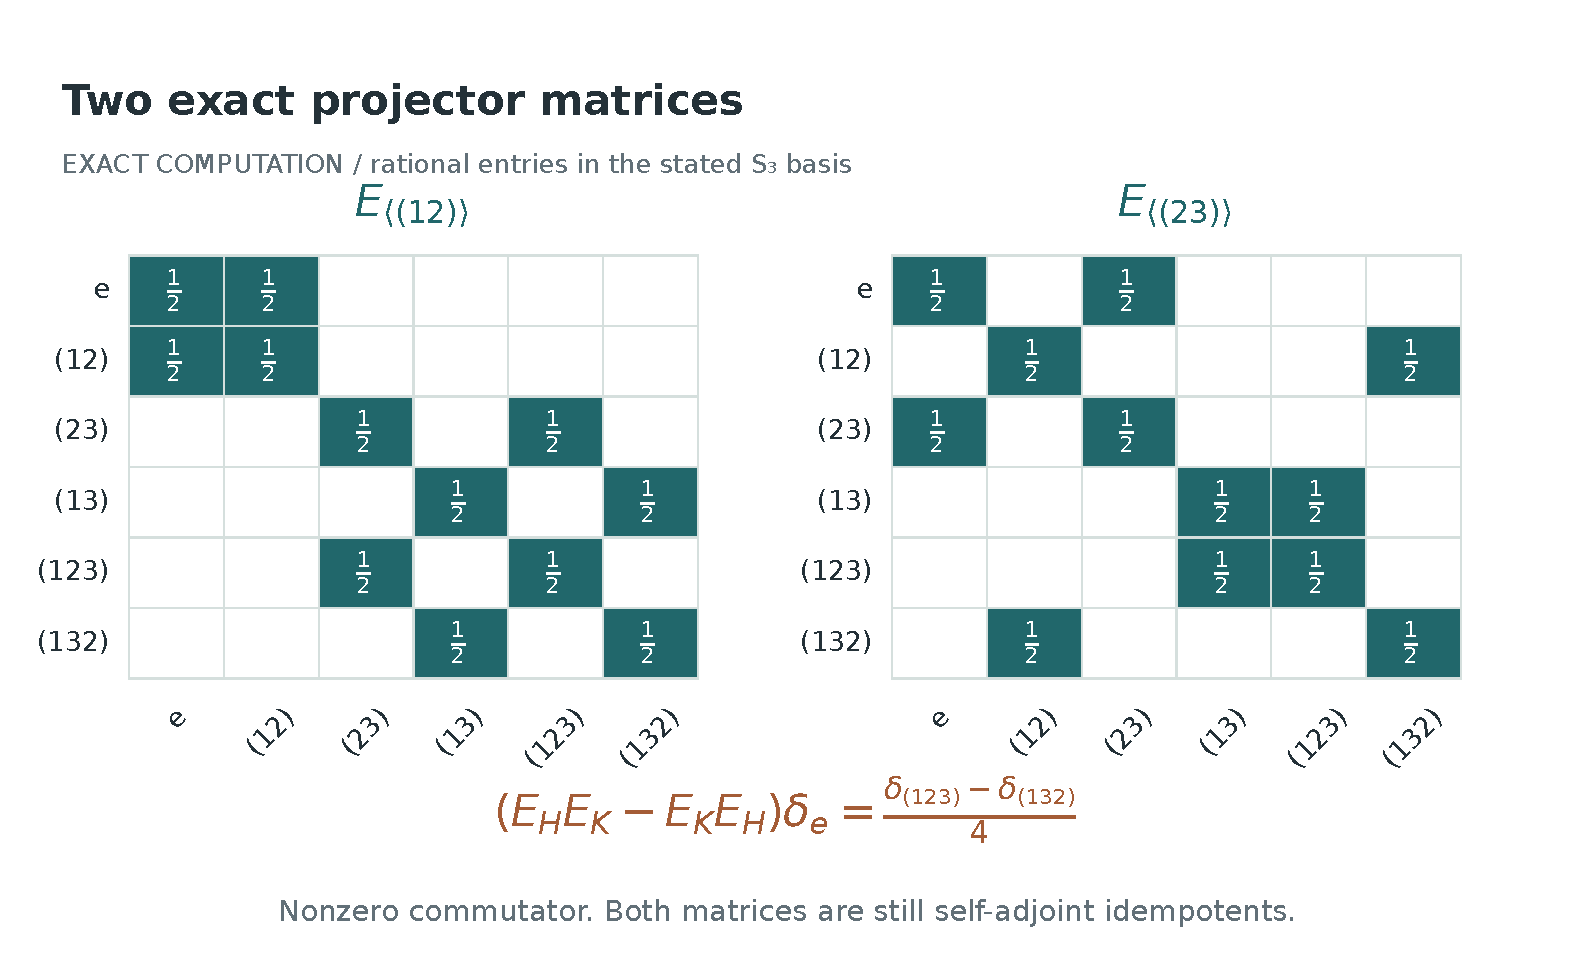
\includegraphics[width=0.96\linewidth]{../visual/figures/12_s3_matrix.pdf}
\caption{Exact \(S_3\) subgroup averages in the declared basis order. The displayed matrices are rational, and the nonzero commutator has squared Hilbert Schmidt norm \(3/4\).}
\label{fig:b-s3-matrix}
\end{figure}

\Needspace{14\baselineskip}
\section{Normality and the meaning of faithful realization}

\begin{theorem}[Normality as central compatibility]
\label{thm:b-normality}
For \(H\leq G\), the following are equivalent in the regular realization:
\begin{enumerate}
\item \(H\) is normal in \(G\).
\item \(e_H\) belongs to the center of \(\C[G]\).
\item \(E_H\) commutes with every \(\lambda(g)\).
\item \(V^H\) is invariant under every \(\lambda(g)\).
\end{enumerate}
When they hold, the action on \(V^H\) factors through a faithful action of \(G/H\).
\end{theorem}

\begin{proof}
Conjugation gives \(ge_Hg^{-1}=e_{gHg^{-1}}\). Equality of these group algebra elements is equality of their supports, hence equality of the subgroups. This proves the equivalence of the first two statements. Injectivity of \(\lambda\) proves equivalence with the third.

An operator commuting with a projection preserves its range. Conversely, if a subspace is invariant under all \(\lambda(g)\), it is invariant under their inverses as well. Since they are unitary, its orthogonal complement is also invariant, so its orthogonal projection commutes with them. This proves the fourth equivalence. Each \(h\in H\) acts trivially on \(V^H\). Normality makes the action on the coset vectors the regular action of \(G/H\), which is faithful by the same argument as \eqref{eq:b-regular-faithfulness}.
\end{proof}

The hypotheses concern an injective representation of the group algebra. A representation can be faithful on group elements while its linear extension kills nonzero group algebra elements. That loss can conceal precisely the supports used by these proofs. The historical phrase faithful realization is therefore read here as the regular realization, or a realization whose group algebra action is injective.

\begin{example}[A faithful group action that hides the boundary]
\label{ex:b-s4-faithfulness}
Let \(S_4\) act by permuting the coordinates of \(\Q^4\), and restrict to
\[
 W=\{(x_1,x_2,x_3,x_4):x_1+x_2+x_3+x_4=0\}.
\]
This standard representation is faithful. Indeed, a permutation acting trivially on \(W\) also acts trivially on the constant line. Their direct sum is \(\Q^4\), so its permutation matrix is the identity.

Take \(r=(1234)\), \(H=\langle r\rangle\), \(k=(12)\), and \(K=\langle k\rangle\). Each coordinate visits all four positions under the cycle, so the average of \(H\) on \(\Q^4\) is the matrix with every entry \(1/4\). Its restriction to \(W\) is zero. Thus the represented average commutes with every operator, including the average of \(K\).

But \(krk=(1342)\) is not among \(1,r,r^2,r^3\), so \(H\) is not normal. Moreover \(kr\in KH\) does not lie in \(HK\). If it equalled \(r^i\), then \(k\in H\), which is false. If it equalled \(r^ik\), then \(krk=r^i\), which is also false. Hence \(HK\ne KH\). Both reverse implications fail in this faithful group action. They hold in the regular action because its group algebra representation retains the missing information.
\end{example}

A trivial representation supplies an even simpler warning: all subgroup averages are the identity. The \(S_4\) example shows that removing the kernel of the group action alone does not cure the problem. What matters is the information retained by the declared realization.

\section{From fixed vectors to fixed fields}

Now suppose an actual finite Galois extension \(L/\Q\) has been given, with group \(G\). The classical correspondence is an external input, in the form stated by Milne \cite[Theorem 3.17]{Milne2022}. It sends \(H\leq G\) to
\[
 L^H=\{x\in L:h(x)=x\text{ for every }h\in H\}.
\]
This is a field because every \(h\) respects sums, products, and inverses. The theorem identifies \(\Gal(L/L^H)=H\), gives \([L^H:\Q]=[G:H]\), and makes subgroup inclusion reverse field inclusion. If \(H\) is normal, it also gives \(\Gal(L^H/\Q)\cong G/H\).

The lattice identities follow directly. An element fixed by both \(H\) and \(K\) is fixed by their generated subgroup, so
\begin{equation}
 L^H\cap L^K=L^{\langle H,K\rangle}.
 \label{eq:b-field-intersection}
\end{equation}
The automorphisms fixing the compositum \(L^HL^K\) are precisely those fixing each field, namely \(H\cap K\). The correspondence then gives
\begin{equation}
 L^HL^K=L^{H\cap K}.
 \label{eq:b-field-compositum}
\end{equation}
These identities require no permutability assumption. The stronger product identity for two averaging operators does require it. A field lattice operation and an ordered composition of linear maps are different operations.

The normal basis theorem supplies a useful translation \cite[Theorem 5.18]{Milne2022}. For some \(\alpha\in L\), the elements \(g(\alpha)\), with \(g\in G\), form a \(\Q\) basis. The map
\begin{equation}
 \Q[G]\longrightarrow L,
 \qquad \sum_g c_g g\longmapsto\sum_g c_g g(\alpha)
 \label{eq:b-normal-basis-map}
\end{equation}
is an equivariant vector space isomorphism. After extending scalars to \(\C\), it transports the regular subgroup averages to the fixed vector spaces of the field action. This verifies the Galois to resolution direction with all its subgroup information preserved.

The map \eqref{eq:b-normal-basis-map} is not generally an algebra isomorphism. A normal basis transports the field multiplication to a bilinear operation on \(\Q[G]\) that depends on \(L\) and on the chosen basis. The usual group algebra multiplication is a different operation. Thus a theorem that identifies the modules has not manufactured a field multiplication, and has not descended a field to \(\Q\).

\section{Trace, norm, and retained multiplication}

In the given finite Galois extension, the normalized fixed projection is
\begin{equation}
 P_H(x)=\frac1{|H|}\sum_{h\in H}h(x)
 =\frac1{|H|}\operatorname{Tr}_{L/L^H}(x).
 \label{eq:b-trace-average}
\end{equation}
The norm is
\begin{equation}
 \operatorname{N}_{L/L^H}(x)=\prod_{h\in H}h(x).
 \label{eq:b-norm-product}
\end{equation}
The sum and product descriptions, together with their tower identities, are classical inputs \cite[Remark 5.47 and Proposition 5.48]{Milne2022}. They show where the resolved formulation has a linear transfer and where it needs a nonlinear transfer.

For a chain \(H\leq K\), the field tower is \(L/L^H/L^K\). Trace and norm compose through that tower. One way to see the formulas is to choose coset representatives for \(K/H\), multiply or sum first over \(H\), and then over the representatives. Every element of \(K\) appears once. Although \(H\) need not be normal in \(K\), the embeddings of \(L^H\) into \(L\) over \(L^K\) are represented by these cosets. This gives
\[
 \operatorname{Tr}_{L/L^K}
 =\operatorname{Tr}_{L^H/L^K}\circ\operatorname{Tr}_{L/L^H},
 \qquad
 \operatorname{N}_{L/L^K}
 =\operatorname{N}_{L^H/L^K}\circ\operatorname{N}_{L/L^H}.
\]
The norm is homogeneous of degree \(|H|\) over the fixed field. It is multiplicative, and generally fails to be additive.

\begin{example}[One projection, different norms]
\label{ex:b-trace-norm-loss}
In \(L=\Q(\sqrt2)\), let \(H\) be the full group. For \(x=a+b\sqrt2\),
\[
 P_H(x)=a,
 \qquad \operatorname{Tr}_{L/\Q}(x)=2a,
 \qquad \operatorname{N}_{L/\Q}(x)=a^2-2b^2.
\]
The elements \(1\) and \(1+\sqrt2\) have the same projection and the same trace, but their norms are \(1\) and \(-1\). There is therefore no function of the projected value alone that recovers the norm on all of \(L\). Similarly, \(P_H(\sqrt2)=0\), while \(P_H((\sqrt2)^2)=2\), so the projection is not multiplicative.
\end{example}

\begin{figure}[tbp]
\centering
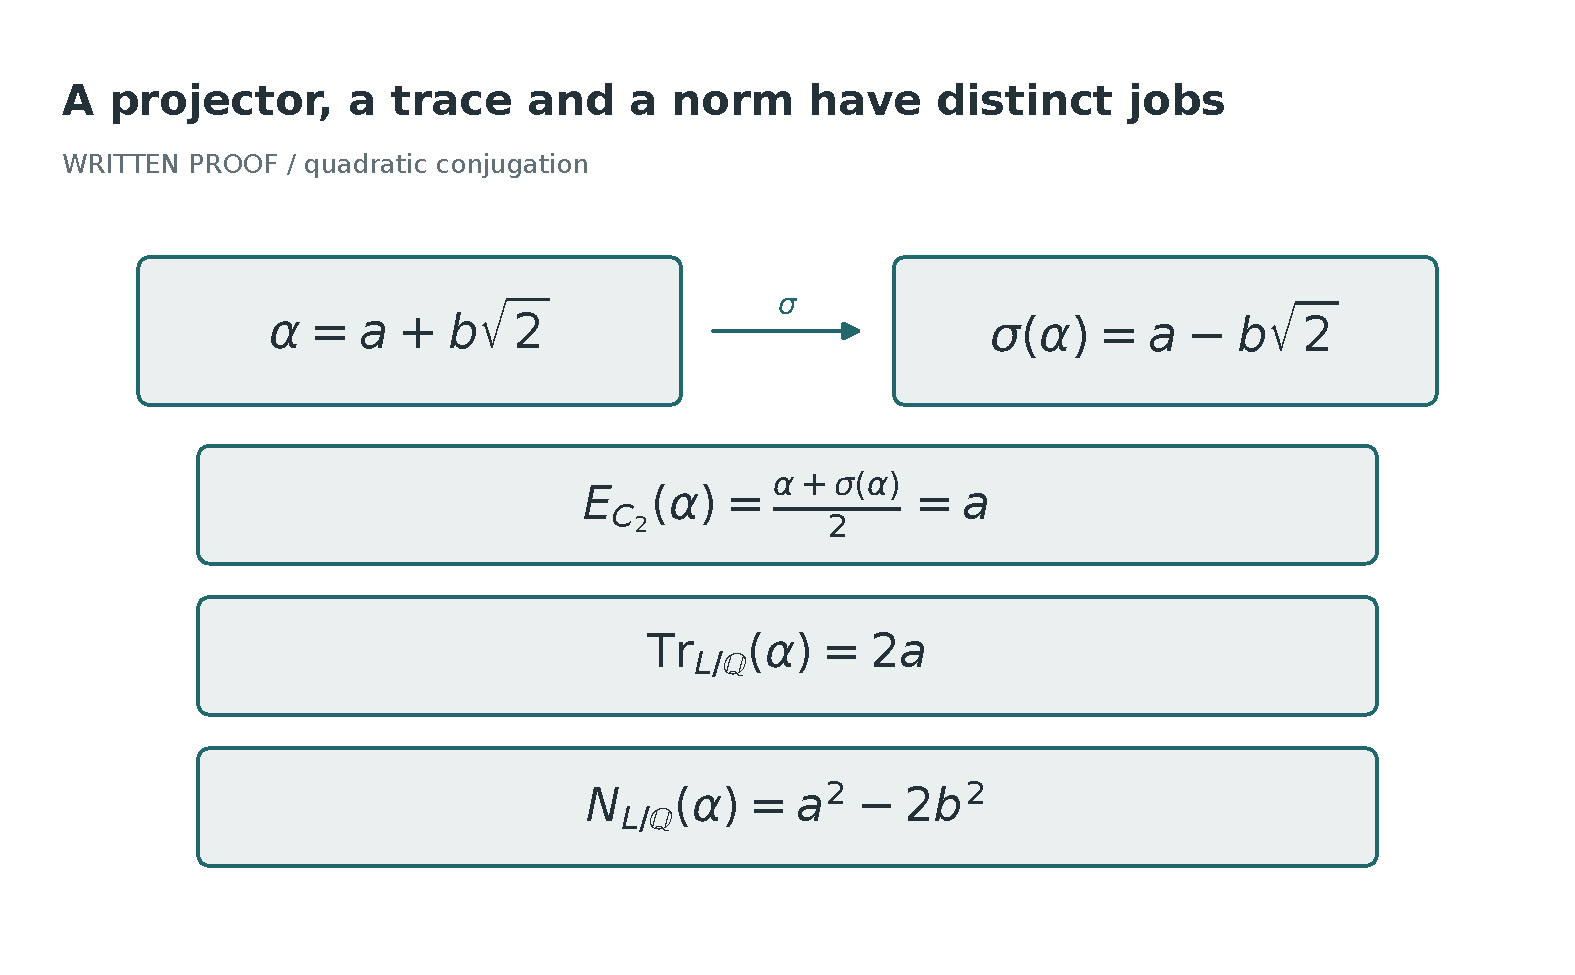
\includegraphics[width=0.96\linewidth]{../visual/figures/15_trace_norm.pdf}
\caption{In \(\Q(\sqrt2)\), averaging retains \(a\), trace retains \(2a\), and norm uses \(a^2-2b^2\). The multiplication and the discarded coordinate affect the norm even when the projected value stays fixed.}
\label{fig:b-trace-norm}
\end{figure}

\begin{claimboundary}
Subgroup averaging, ranks, compatibility, and normality have been proved for the regular module of every finite group. Classical Galois theory translates an already given field extension into that module language. The translation retains the field only when its multiplication and arithmetic base remain part of the object. A regular representation by itself supplies neither of them.
\end{claimboundary}

\addtocontents{toc}{\protect\newpage}
\chapter{A regular family and the specialization step}
\label{ch:regular-specialization}

The inverse Galois problem has a strong geometric route. First construct a family over \(\Q(t)\) with the desired finite Galois group. Then choose a rational parameter whose specialization retains the whole group. The second step is supplied by Hilbert irreducibility under precise hypotheses. The first step contains substantial arithmetic work. Treating the second step as automatic existence of the family would reverse the logical direction of the theorem.

\section{What regularity asks for}

Let \(t\) be transcendental over \(\Q\). A finite Galois extension \(F/\Q(t)\) is regular over \(\Q\) when \(\Q\) is algebraically closed in \(F\). Equivalently in the present characteristic zero setting,
\begin{equation}
 F\cap\overline{\Q}=\Q,
 \label{eq:b-regular-constants}
\end{equation}
inside an algebraic closure containing both fields. This condition excludes an extension obtained solely by enlarging the constants. It permits the family to remain connected over an algebraic closure of the constant field. The terminology and the implication from regular to ordinary realization over a Hilbertian base are documented in D\`ebes and Harbater \cite[Introduction]{DebesHarbater2021}.

If \(L/\Q\) is a nontrivial finite Galois extension, adjoining a dummy variable gives \(L(t)/\Q(t)\) with the same abstract group. It contains every element of \(L\) as an algebraic constant, so it is not regular. An ordinary realization therefore does not yield a regular one by this particular construction. The existence of a regular realization for every finite group is a stronger proposed input. This chapter uses no converse from ordinary realization to regular realization.

Regularity can be inspected only after the family is a field with a specified base. A matrix action depending on a symbol \(t\) does not by itself define \(F\). One needs equations or another construction of the extension, its connectedness, its arithmetic constant field, and the group of the full splitting field. These properties are part of the input to specialization.

\section{The exact specialization contract}

\begin{theorem}[Hilbert specialization, external input]
\label{thm:b-hilbert-specialization}
Let \(F/\Q(t)\) be a finite Galois field extension with group \(G\). After choosing a suitable model and excluding the finitely many zeros of a nonzero constraint polynomial, there are infinitely many rational values \(a\) for which a specialization has Galois group isomorphic to \(G\). In particular, an actual regular \(G\) extension of \(\Q(t)\) gives a \(G\) extension of \(\Q\).
\end{theorem}

This is the one parameter form of the checked Hilbert specialization contract. The source proof uses a primitive element for the entire Galois extension, a Hilbert subset preserving its irreducibility, and a localization avoiding coefficients, denominators, and discriminant zeros \cite[Theorem 2.6.3, Theorem 5.2.4 and Proposition 5.2.14]{DebesLectureNotes}. The regular consequence over \(\Q\) is also stated in the checked recent preprint \cite[Section 1.2]{HuangEtAl2026}. These are external theorem inputs. The present manuscript does not replace their proofs with a finite sample of parameter values.

The degree bookkeeping explains the conclusion. A primitive polynomial for \(F\) has degree \([F:\Q(t)]=|G|\). At suitable values its specialization remains irreducible of that degree. Away from the excluded model locus, specialization supplies a group inside the original \(G\). Preserving the full extension degree forces the specialized group to have \(|G|\) elements, hence to be the full group. A polynomial defining only one root field can have smaller degree, so preserving that polynomial's irreducibility alone is not this full degree argument.

\begin{corollary}[Conditional realization route]
\label{cor:b-regular-route}
For a prescribed finite group \(G\), a verified regular finite Galois extension \(F/\Q(t)\) with group \(G\), followed by Theorem~\ref{thm:b-hilbert-specialization}, proves an ordinary realization of \(G\) over \(\Q\).
\end{corollary}

\begin{proof}
Apply the external theorem to that extension, and choose one of the suitable rational parameters outside the finite excluded set. Its specialized field is the required finite Galois extension of \(\Q\).
\end{proof}

The theorem gives existence of suitable parameters. It does not identify every allowed parameter as suitable, nor does it automatically give a short search or a bound on the discriminant. A parameter outside the branch locus may still specialize to a smaller group. These are different questions: the model can be nonsingular at a value while the resulting polynomial acquires extra factorization over \(\Q\).

In several parameters, the excluded set is a proper algebraic locus and may be infinite. In one parameter, a nonzero polynomial has finitely many roots, which is why the finite exceptional set wording is appropriate here. The base \(\Q\) is also essential to the source contract. Characteristic zero by itself does not imply Hilbert irreducibility. For instance, over \(\C\) every specialization of a nonconstant irreducible polynomial in \(X\) splits into linear factors, so the required retention of a degree greater than one fails.

\begin{figure}[tbp]
\centering
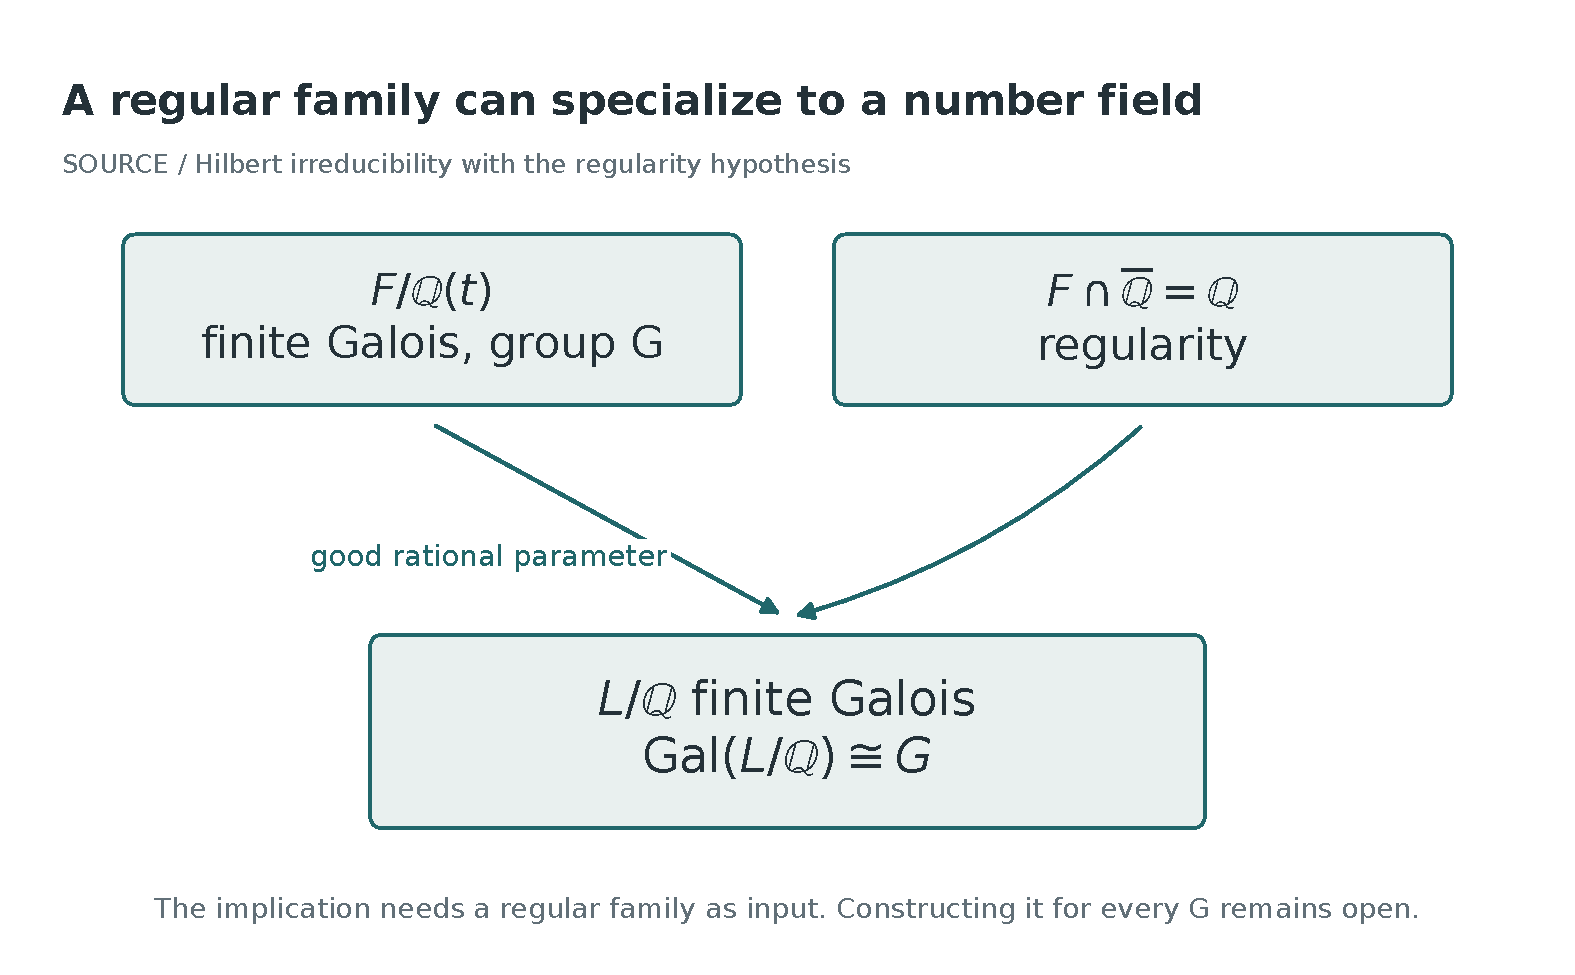
\includegraphics[width=0.96\linewidth]{../visual/figures/16_regular_specialization.pdf}
\caption{The specialization theorem starts with a verified arithmetic family. The suitable rational parameter belongs to a Hilbert subset and avoids the chosen model's exceptional values. Both conditions appear in the inference to a field over \(\Q\).}
\label{fig:b-regular-specialization}
\end{figure}

\section{A cubic toy that changes group}

The polynomial
\begin{equation}
 f_t(X)=X^3-t
 \label{eq:b-cubic-family}
\end{equation}
is a small exact example of what can happen under specialization. It is used here to study changes in the splitting field group. Its generic splitting field is not a regular extension of \(\Q(t)\), a fact established below.

At \(t=2\), the polynomial \(X^3-2\) is irreducible by Eisenstein at the prime \(2\). Let \(\alpha=\sqrt[3]{2}\) be the real root and let \(\zeta\) be a primitive cube root of unity. The splitting field is
\[
 L_2=\Q(\alpha,\zeta).
\]
The real field \(\Q(\alpha)\) has degree three. It cannot contain the nonreal element \(\zeta\). Adjoining \(\zeta\), whose minimal polynomial is \(X^2+X+1\), therefore doubles the degree. The splitting field has degree six and its faithful action on the three roots identifies its group with \(S_3\). Equivalently, the discriminant is \(-27\cdot2^2=-108\), which is not a rational square. The classical irreducible cubic criterion is checked in Milne \cite[Proposition 4.5 and Example 4.7]{Milne2022}.

At \(t=1\),
\[
 X^3-1=(X-1)(X^2+X+1).
\]
The splitting field is \(\Q(\zeta)\), of degree two, with group \(C_2\). The discriminant \(-27\) is nonzero, so this is an unbranched parameter for the simple discriminant test, yet the group has dropped from \(S_3\). At \(t=0\), the polynomial becomes \(X^3\), with a repeated root, and its splitting field is simply \(\Q\). That value lies on the discriminant zero locus. Thus the toy separates a singular degeneration from a nonsingular group drop.

The generic splitting field also has group \(S_3\). To prove this without an experimental inference, take a transcendental \(u\) and put \(t=u^3\). The polynomial \(X^3-t\) is Eisenstein at the prime \(t\) in \(\Q[t][X]\), hence irreducible over \(\Q(t)\). Its root field is \(\Q(u)\), and the splitting field is \(\Q(u,\zeta)\). The only elements of \(\Q(u)\) algebraic over \(\Q\) lie in \(\Q\). Indeed, if a nonconstant rational function \(v(u)\) were algebraic over \(\Q\), clearing the equation defining \(v\) would make \(u\) algebraic over \(\Q(v)\), contradicting its transcendence. Hence \(\zeta\notin\Q(u)\). The generic extension again has degree six and group \(S_3\).

However, its constant field contains \(\Q(\zeta)\), so it violates \eqref{eq:b-regular-constants}. It cannot serve as the worked regular input of Corollary~\ref{cor:b-regular-route}. The valid conclusions are the three specialization computations and the explicit generic group calculation. The general specialization theorem also admits nonregular finite Galois inputs under its stated model hypotheses, but their specializations need not give infinitely many distinct field isomorphism classes. A constant extension illustrates why suitable parameter values and distinct extensions should not be identified without an additional argument.

\begin{figure}[tbp]
\centering
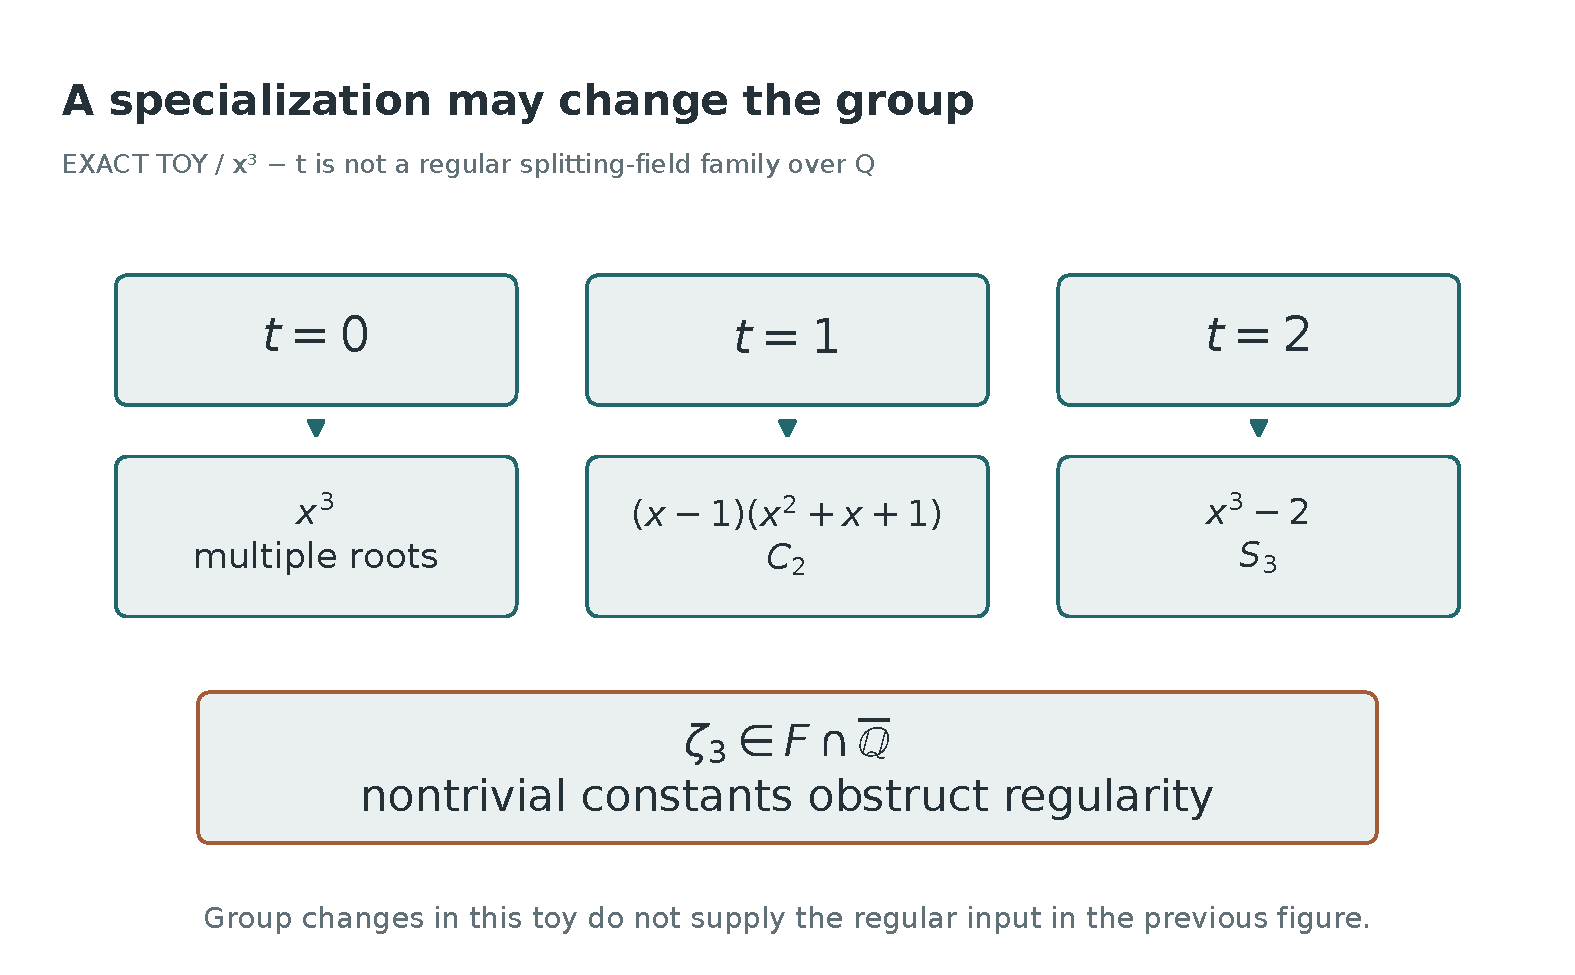
\includegraphics[width=0.96\linewidth]{../visual/figures/17_parameter_bad.pdf}
\caption{The specialization toy \(X^3-t\) has group \(S_3\) at \(t=2\), group \(C_2\) at the nonsingular value \(t=1\), and trivial splitting field at \(t=0\). Its generic splitting field contains \(\zeta_3\), so this is not a regular family over \(\Q\).}
\label{fig:b-parameter-toy}
\end{figure}

\section{Geometric existence and arithmetic descent}

A construction over \(\C(t)\) has a different base from one over \(\Q(t)\). Even if it comes from an exact complex cover with the intended group, the construction still needs an arithmetic model over \(\Q\), together with compatible equations and descent data. An action on its geometric fibers does not by itself prove that this model exists over the smaller base.

The elementary constant example already displays the issue. The equation \(X^3-t\) has cyclic splitting field over \(\C(t)\), since \(\zeta_3\) is in the base. Over \(\Q(t)\), its splitting field has group \(S_3\), with an extra arithmetic action on that constant. Passing between bases can change the group being discussed. For a regular arithmetic family, one must verify the stated arithmetic group and the absence of enlarged constants, rather than assigning the geometric group to both settings by notation.

This is where the packet language can record a useful obligation. A geometric construction may organize branch behavior, group actions, and local charts. An arithmetic descent claim asks that its chart transitions and coefficients arise from an effective object over \(\Q\). A specialization claim then starts from that object. Keeping the two steps separate prevents a valid complex construction from being promoted into an unsupported rational realization.

\begin{openproblem}
For the general regular route, the missing input is a verified regular \(G\) extension over \(\Q(t)\) for each prescribed finite group \(G\). Hilbert specialization applies after that input has been constructed. A complex cover, a regular module, or a compatible system of projectors does not establish the required arithmetic descent by itself.
\end{openproblem}

\chapter{Embedding problems and the lift that must be proper}
\label{ch:embedding-problems}

An embedding problem makes the realization obstruction relative. Suppose one finite Galois extension has already been found. Can it be enlarged so that a prescribed extension of its group appears as the full new Galois group? This asks for more than constructing an abstract extension of finite groups. The new group must be reached by a continuous quotient of the absolute Galois group, and the quotient must respect the existing field.

\section{The diagram and its fields}

Fix an algebraic closure \(\overline\Q\), and write
\[
 G_{\Q}=\Gal(\overline\Q/\Q)
\]
with its Krull topology. For a finite Galois subfield \(L\subset\overline\Q\), restriction supplies a continuous epimorphism \cite[Proposition 7.7]{Milne2022}
\[
 \rho:G_{\Q}\longrightarrow G=\Gal(L/\Q).
\]
Now specify an exact sequence of finite groups
\begin{equation}
 1\longrightarrow N\longrightarrow E\overset{\pi}{\longrightarrow}G\longrightarrow1.
 \label{eq:b-group-extension}
\end{equation}
The finite targets carry the discrete topology. A solution is a continuous homomorphism
\begin{equation}
 \widetilde\rho:G_{\Q}\longrightarrow E,
 \qquad \pi\circ\widetilde\rho=\rho.
 \label{eq:b-lift-equation}
\end{equation}
It is a weak solution when this equation holds, and a proper solution when \(\widetilde\rho\) is also surjective.

Continuity is part of the definition. For a finite discrete target it makes the kernel open. The fixed field of that kernel is therefore a finite Galois extension of \(\Q\), with group equal to the image of the map. These facts belong to the classical absolute Galois correspondence \cite[Theorem 7.13]{Milne2022}. They explain why a homomorphism without the continuity hypothesis is not the required arithmetic certificate.

Let \(J=\widetilde\rho(G_{\Q})\leq E\). Even a weak solution satisfies \(\pi(J)=G\), since \(\rho\) is onto. The inclusion \(\ker\widetilde\rho\subseteq\ker\rho\) gives a finite Galois field \(M\) containing \(L\). Its group is \(J\), rather than necessarily \(E\). Properness makes the exact arithmetic tower
\[
 \Gal(M/\Q)\cong E,
 \qquad \Gal(M/L)\cong N,
 \qquad \Gal(L/\Q)\cong G.
\]
The quotient map in this tower must be the specified \(\pi\) under these identifications.

\begin{figure}[tbp]
\centering
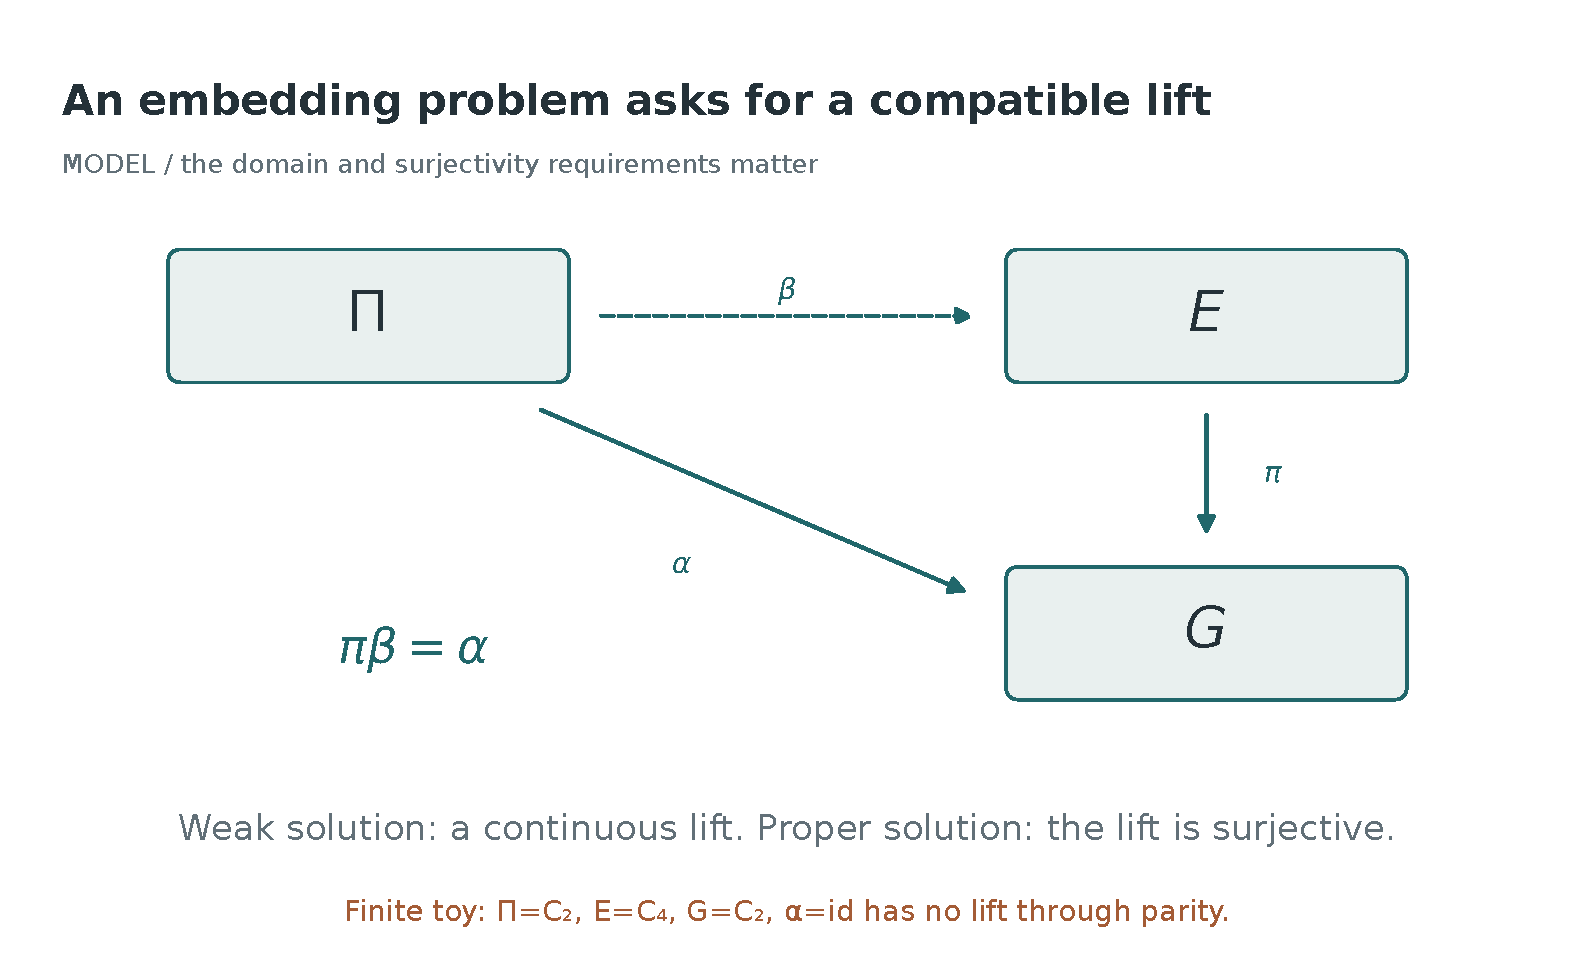
\includegraphics[width=0.96\linewidth]{../visual/figures/18_embedding_problem.pdf}
\caption{An embedding problem fixes the quotient map \(\pi:E\to G\) and the existing arithmetic quotient \(\rho:G_{\Q}\to G\). The lift must be continuous, must make the triangle commute, and must be surjective to be proper.}
\label{fig:b-embedding-problem}
\end{figure}

\section{A finite no lift toy}

The following example is an exact finite group calculation. Its domain is the finite group \(C_2\), rather than \(G_{\Q}\). It is useful because it isolates an obstruction to lifting a relation.

\begin{example}[The identity of \(C_2\) does not lift to \(C_4\)]
\label{ex:b-no-lift}
Use additive notation and take
\[
 \Gamma=\Z/2\Z,
 \quad E=\Z/4\Z,
 \quad G=\Z/2\Z,
 \quad \pi(x)=x\bmod2,
 \quad \rho=\operatorname{id}_{\Gamma}.
\]
If \(\widetilde\rho:\Gamma\to E\) were a lift, the image \(y\) of the nonzero element would satisfy \(\pi(y)=1\), so \(y\) would be \(1\) or \(3\) modulo four. But the relation \(1+1=0\) in \(\Gamma\) forces \(2y=0\) in \(E\), which holds only for \(y=0\) or \(2\). No such lift exists.
\end{example}

The surjection \(C_4\to C_2\) is perfectly valid, and each element of \(C_2\) has a preimage. The failure occurs when the preimages must respect the domain's group law. Lifting individual elements is therefore weaker than lifting the homomorphism. An arithmetic construction must respect all relations and its continuity requirements at once.

This toy is not a counterexample to solvability of an absolute Galois embedding problem with the same finite targets. Its proof uses the order two relation in the chosen finite domain. The absolute Galois group is a different domain, and an arithmetic quotient may be reached through elements and relations that are absent from this toy. The example supplies a precise warning about an invalid inference, not a general arithmetic impossibility theorem.

\section{A split lift can still be weak}

An extension splits when \(\pi\) has a homomorphic section \(s:G\to E\). For such a section, \(s\circ\rho\) is automatically a continuous weak solution: \(\rho\) is continuous by hypothesis, \(s\) is continuous between finite discrete groups, and \(\pi s\rho=\rho\). Its image is \(s(G)\). If the kernel \(N\) is nontrivial, this image has order \(|G|<|E|\), so that particular solution is not proper.

\begin{example}[The kernel is missed in a direct product]
\label{ex:b-split-weak}
Take \(E=N\times G\) with \(\pi(n,g)=g\). The section \(s(g)=(1,g)\) gives
\[
 \widetilde\rho_0(\gamma)=(1,\rho(\gamma)).
\]
Its image is \(\{1\}\times G\). It reaches every element of the desired quotient, but reaches none of the nonidentity elements of \(N\times\{1\}\). With the finite toy \(N=G=\Gamma=C_2\) and \(\rho\) the identity, the image has two elements while \(E\) has four. All lift equations hold, and properness fails.
\end{example}

\begin{proposition}[Exact kernel coverage criterion]
\label{prop:b-kernel-coverage}
Let \(\Gamma\) be any group, let \(\rho:\Gamma\to G\) be onto, and let \(\widetilde\rho:\Gamma\to E\) be a homomorphic lift through \eqref{eq:b-group-extension}. Then \(\widetilde\rho\) is onto if and only if
\begin{equation}
 \widetilde\rho(\ker\rho)=N.
 \label{eq:b-kernel-coverage}
\end{equation}
\end{proposition}

\begin{proof}
Every image of \(\ker\rho\) lies in \(N\). If \(\widetilde\rho\) is onto, every \(n\in N\) has a preimage \(\gamma\), and \(\rho(\gamma)=\pi(n)=1\), proving the equality. Conversely, assume the equality and take \(e\in E\). Surjectivity of \(\rho\) gives \(\gamma\) with \(\rho(\gamma)=\pi(e)\). Then \(e\widetilde\rho(\gamma)^{-1}\in N\). By the hypothesis it equals \(\widetilde\rho(\delta)\) for some \(\delta\in\ker\rho\). Hence \(e=\widetilde\rho(\delta\gamma)\), proving surjectivity.
\end{proof}

This criterion gives an exact remaining task after a weak solution is found. The quotient has already been covered. Properness asks whether the arithmetic kernel supplies the full additional group. A computation of the quotient action alone cannot answer that question.

For a direct product, a candidate lift has the form \((\eta,\rho)\), where \(\eta:\Gamma\to N\) is a homomorphism. Even surjectivity of both coordinates does not automatically imply surjectivity of the pair. If \(\Gamma=N=G=C_2\) and both maps are the identity, their combined image is the diagonal subgroup of order two. Proposition~\ref{prop:b-kernel-coverage} locates the failure: the kernel of \(\rho\) is trivial and supplies no nontrivial kernel element.

\begin{figure}[tbp]
\centering
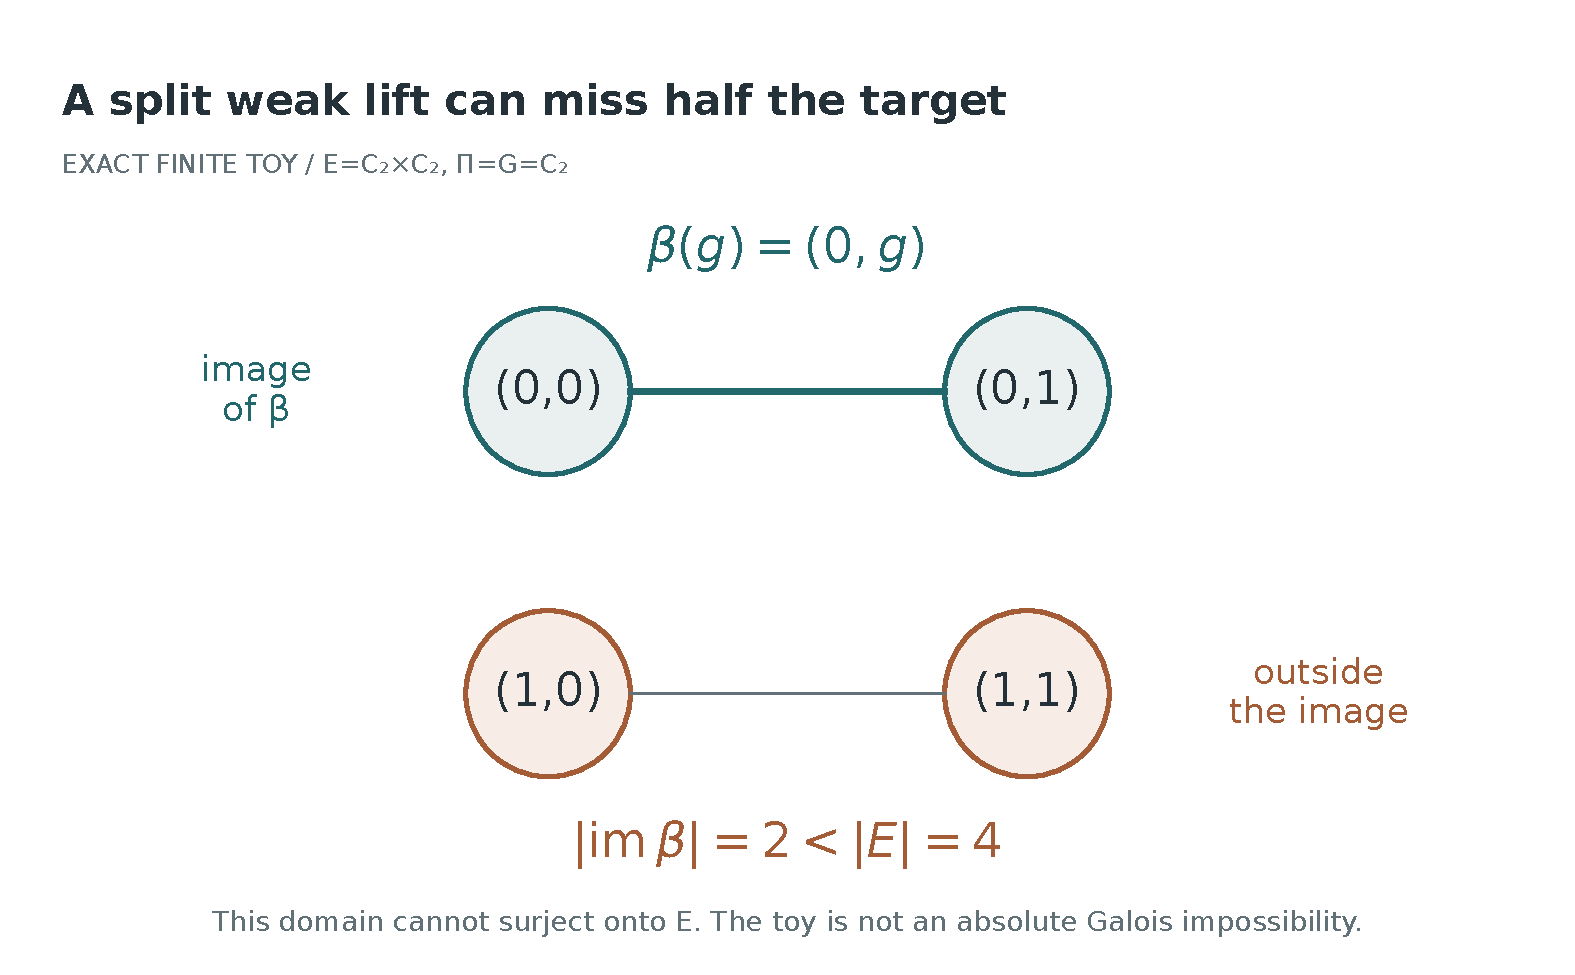
\includegraphics[width=0.96\linewidth]{../visual/figures/19_weak_proper.pdf}
\caption{A weak solution can cover the quotient while missing the extension kernel. Properness requires exactly \(\widetilde\rho(\ker\rho)=N\), in addition to the commuting lift equation. The finite split example illustrates this distinction.}
\label{fig:b-weak-proper}
\end{figure}

\FloatBarrier
\section{The relation defect of a chosen section}

A set theoretic section may select preimages without being a homomorphism. Its failure to preserve products is an exact defect. To state the calculation cleanly, assume here that \(N\) is central in \(E\). Centrality makes \(N\) abelian. Choose a section \(s:G\to E\) with \(s(1)=1\), and define
\begin{equation}
 c(g,h)=s(g)s(h)s(gh)^{-1}\in N.
 \label{eq:b-section-defect}
\end{equation}
Associativity in \(E\) gives
\begin{equation}
 c(g,h)c(gh,k)=c(h,k)c(g,hk),
 \label{eq:b-cocycle-law}
\end{equation}
because central elements can be moved past the section values. The normalized identities are \(c(1,g)=c(g,1)=1\). Thus the defect is a central two cocycle, with its law proved by the group multiplication itself.

\begin{proposition}[Explicit central lift equation]
\label{prop:b-central-lift}
For a homomorphism \(\rho:\Gamma\to G\), a lift has the form
\begin{equation}
 \widetilde\rho(\gamma)=u(\gamma)s(\rho(\gamma)),
 \qquad u(\gamma)\in N.
 \label{eq:b-corrected-section}
\end{equation}
It is a homomorphism if and only if \(u(1)=1\) and
\begin{equation}
 u(\gamma\delta)
 =u(\gamma)u(\delta)c(\rho(\gamma),\rho(\delta))
 \quad(\gamma,\delta\in\Gamma).
 \label{eq:b-correction-equation}
\end{equation}
For a topological domain and finite targets, the lift is continuous if and only if \(u\) is continuous, provided \(\rho\) is continuous.
\end{proposition}

\begin{proof}
Any lift differs from \(s\rho\) by a unique element of the kernel, giving \eqref{eq:b-corrected-section}. Centrality and \eqref{eq:b-section-defect} give
\[
 \widetilde\rho(\gamma)\widetilde\rho(\delta)
 =u(\gamma)u(\delta)c(\rho(\gamma),\rho(\delta))s(\rho(\gamma\delta)).
\]
Comparison with the expression for \(\widetilde\rho(\gamma\delta)\) proves the equivalence. The identity condition makes the identity map correctly. Since a map between finite discrete sets is continuous, \(s\rho\) is continuous whenever \(\rho\) is. The equation relating \(u\) and \(\widetilde\rho\) then proves both directions of the continuity assertion.
\end{proof}

This proposition states the obstruction without assuming it disappears. A successful correction \(u\) removes the pulled back defect in the stated multiplicative convention. In cohomological terminology this is the triviality of the corresponding pulled back class. Such triviality needs a proof for the actual arithmetic quotient and kernel action. For a noncentral kernel, conjugation introduces a nontrivial action and changes the correction equation. The central formula cannot be used unchanged there.

The finite \(C_4\) example also appears in these coordinates. In additive notation select \(s(0)=0\), \(s(1)=1\). The defect at \((1,1)\) is \(2\) modulo four. A correction \(u(1)\) must be in the kernel \(\{0,2\}\). Equation~\eqref{eq:b-correction-equation} then becomes
\[
 0=2u(1)+2\pmod4,
\]
which is impossible. This reproduces the order obstruction using a relation defect. It is an exact finite computation and an exact finite proof. It supplies no assertion that an analogous class always vanishes or always persists over \(G_{\Q}\).

\section{What closes an arithmetic embedding problem}

For a specific arithmetic problem, the required certificate has three layers. First the starting map \(\rho\) must come from the declared finite Galois extension. Second a continuous lift must solve the exact relation equation for the chosen group extension, with all actions and descent data specified. Third the image must be the full group \(E\), equivalently the arithmetic kernel must cover \(N\).

A projector construction can faithfully encode the finite targets and their quotient action. It can also keep a residual for a failed relation or a missed kernel direction. That is useful evidence about the construction. It becomes an arithmetic existence proof only when the corrected data define the required continuous quotient and its finite fixed field. The source theorem realizing finite solvable groups over \(\Q\) is a substantial external existence result \cite[Theorem 1]{SchmidtWingberg1998}. It cannot be substituted for an unchecked claim that every specified embedding problem, with every prescribed local condition, has a proper solution.

The same care applies to descent. Matching a finite collection of matrices can prove a compatibility identity within their realized vector spaces. Effective descent requires the identity to be part of a complete object over the intended field, including its coefficients and multiplication. A local chart repair may remove one visible defect while leaving another arithmetic obstruction. The resolved language helps by naming those separate obligations rather than treating a zero matrix residual as the end of every existence problem.

\begin{claimboundary}
The finite lift obstruction, the split weak lift, the kernel coverage criterion, and the central correction equation have complete arguments in this chapter. They organize the remaining arithmetic task. They do not prove that every embedding problem over \(G_{\Q}\) has a proper solution, and they do not close the unrestricted inverse Galois conjecture.
\end{claimboundary}

\chapter{A certificate that contains an actual field}
\label{chap:g07-certificate}

\section{What an inverse construction must return}

The preceding chapters provide several exact objects attached to a finite group. A multiplication table determines the group. Its regular representation determines a family of rational permutation matrices. Its subgroups determine averaging projectors. The variable construction supplies a finite Galois extension over an invariant field. Each output has a definite mathematical type. The inverse Galois target requires a finite field over $\Q$.

One useful way to express the remaining task is to specify a certificate that would finish it for a chosen group. The specification makes no assertion that the certificate is easy to find. It states what a proposed construction must contain before the arithmetic conclusion follows.

Let $G$ be a finite group of order $n$. A polynomial field presentation consists of a monic irreducible polynomial $f\in\Q[X]$ of degree $n$ and
\[
 L=\Q[X]/(f),\qquad \theta=X\bmod f.
\]
Irreducibility is the field input. The quotient is automatically a commutative algebra of dimension $n$, but that dimension alone would also hold for a reducible polynomial. A reducible quotient can have zero divisors or nilpotents and cannot serve as the requested field.

For every $g\in G$, specify a polynomial $r_g\in\Q[X]$ of degree less than $n$. It is intended to describe $\sigma_g(\theta)=r_g(\theta)$. The equality
\[
 f(r_g(\theta))=0
\]
ensures that this substitution induces a unital $\Q$-algebra endomorphism of $L$. Because $L$ is a field, the endomorphism is injective. Because it is a linear endomorphism of a finite dimensional vector space, it is surjective. Thus it is an automorphism.

The group law must still hold. With our convention that $\sigma_g\sigma_h$ means apply $\sigma_h$ first, the required congruences are
\begin{align}
 r_1(X)&\equiv X\pmod f,\label{eq:g07-unit}\\
 r_h(r_g(X))&\equiv r_{gh}(X)\pmod f.\label{eq:g07-composition}
\end{align}
The reversed order of the displayed polynomial substitutions is deliberate. Applying $\sigma_g$ to $r_h(\theta)$ replaces $\theta$ by $r_g(\theta)$, since rational coefficients are fixed. Finally the residues $r_g\bmod f$ must be pairwise distinct. Equal generator images would give equal automorphisms and could collapse the intended group.

\begin{theorem}[Finite field realization certificate]
\label{thm:g07-certificate}
Suppose $f$ and $(r_g)_{g\in G}$ satisfy the field, root, composition and distinctness conditions above. Then $L/\Q$ is finite Galois and
\[
 \Gal(L/\Q)\simeq G.
\]
\end{theorem}

\begin{proof}
The substitutions give a homomorphism from $G$ into $\Aut_{\Q}(L)$. The identity and composition congruences prove the homomorphism law. Distinct generator images make the homomorphism injective. Write its image as $\Sigma$, so $|\Sigma|=n$.

Apply the finite automorphism fixed-field theorem, in the form recorded in source contract LC10. It gives a finite Galois extension $L/L^\Sigma$ with
\[
 [L:L^\Sigma]=|\Sigma|=n,
 \qquad \Gal(L/L^\Sigma)=\Sigma.
\]
All substitutions fix $\Q$, hence $\Q\subseteq L^\Sigma$. Since $[L:\Q]=\deg f=n$, the degree formula gives
\[
 n=[L:L^\Sigma][L^\Sigma:\Q]
   =n[L^\Sigma:\Q].
\]
Therefore $L^\Sigma=\Q$. The preceding Galois assertion now has the required rational base, and the full group is $\Sigma\simeq G$.
\end{proof}

The theorem is a sufficient certificate, not a restriction on what a genuine realization may look like. Every finite Galois extension in characteristic zero has a primitive element. A realization of $G$ has degree $|G|$, and each automorphism's image of that element has a unique expression in the power basis. Thus an existing realization can be written in this format. The primitive element theorem is the classical input, rather than a new search procedure \cite[Theorem 5.1]{Milne2022}.

\section{An exact quadratic certificate}

For $G=C_2=\{1,s\}$, take $f=X^2-2$ and choose
\[
 r_1=X,\qquad r_s=-X.
\]
The polynomial is irreducible over $\Q$, because two is not a rational square. Both residues satisfy $f(r_g)\equiv0\pmod f$. The nontrivial composition gives $r_s(r_s(X))=X$, and the two images are distinct. The certificate theorem returns $\Q(\sqrt2)/\Q$ with its full group $C_2$.

This example shows why the certificate has several checks. The substitution $r_s=X$ would still preserve the polynomial but would fail distinctness. The same pair of substitutions with $f=X^2-1$ would pass root and composition calculations but fail the field condition. One cannot replace irreducibility by an appealing symmetry of the roots.

\section{The multiplication carried by a normal basis}

The normal basis theorem supplies a regular module for an already existing finite Galois extension \cite[Theorem 5.18]{Milne2022}. If $L/\Q$ has group $G$ and normal basis generator $\alpha$, the vector-space map
\[
 \Phi:\Q[G]\longrightarrow L,
 \qquad \sum_g a_g g\longmapsto\sum_g a_g g(\alpha)
\]
is an equivariant linear isomorphism. It transfers subgroup averages and their fixed vector spaces. It is not a claim that the usual multiplication in $\Q[G]$ is field multiplication.

The transported multiplication is a bilinear map
\[
 \mu:\Q[G]\otimes_\Q\Q[G]\longrightarrow\Q[G],
 \qquad \mu(u,v)=\Phi^{-1}(\Phi(u)\Phi(v)).
\]
For the left regular action $\lambda$, it obeys
\[
 \lambda(g)\mu(u,v)=\mu(\lambda(g)u,\lambda(g)v).
\]
It is associative and commutative, has a unit and has no zero divisors. Its coefficients depend on the field and on the chosen normal basis. The normal basis theorem assumes that field before producing the basis. It cannot be used backwards to infer that an arbitrary choice of these coefficients has all the required properties.

The coordinate algebra $\Q^G$ provides a precise comparison. Its pointwise product is equivariant under regular translation, associative, commutative and unital. The invariant subalgebra consists of constant functions, so it is $\Q$. Nevertheless, two different coordinate idempotents multiply to zero. This algebra satisfies many visible symmetry and fixed-object conditions while failing the field condition. For a nontrivial $G$, it is a disconnected algebra rather than a number field.

A coordinate construction must supply a rational multiplication tensor defining a field, verify that the prescribed action preserves it, and identify the full rational automorphism group. The certificate above records these obligations.

\begin{figure}[tbp]
\centering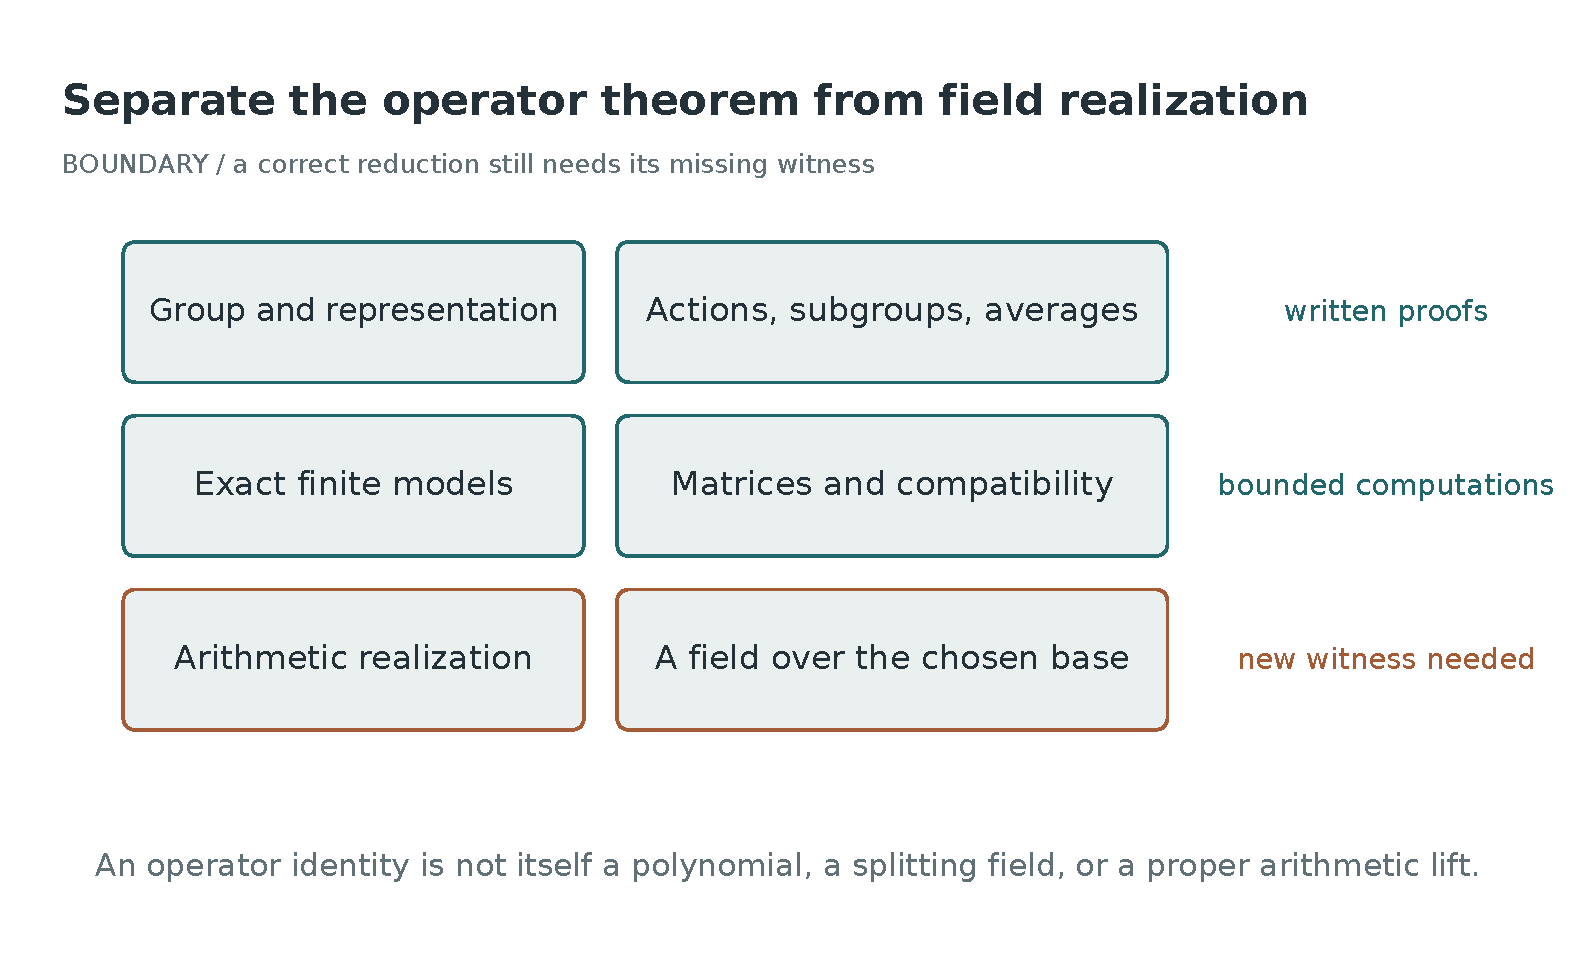
\includegraphics[width=0.85\linewidth]{../visual/figures/20_boundary.pdf}
\caption{Finite symmetry can describe different objects. The inverse Galois target requires a number field over $\Q$ with exactly the prescribed full automorphism group.}
\label{fig:g07-boundary}
\end{figure}

\section{Finding and verifying are different tasks}

Given rational candidates, root and composition tests use exact polynomial remainders, and distinctness uses reduced residues. Irreducibility still needs an exact field certificate, for example a suitable modular argument.

These checks can reject a reducible quotient, a collapsed action or an incorrect fixed base. Passing them for one group does not construct candidates for every group or give a uniform time or size bound.

The finite checks cover five polynomials, all 36 ordered pairs of six $S_3$ subgroups, a faithful $S_4$ boundary and two lift models. Their scope is these examples.

\chapter{The remaining realization program}
\label{chap:g08-program}

\section{What this edition closes}

The five field examples are complete realizations of their specified groups. Their proofs account for field degree, separability and the full splitting-field group. The projector arguments are universal statements in their declared regular representation. The finite lifting examples distinguish compatibility from properness. The certificate theorem turns explicit rational field data into a full realization statement.

The larger uniform routes remain conditional at identifiable points. The variable action realizes every finite group over its invariant field. A rational parametrization of that invariant field would allow Hilbert specialization. A regular realization over $\Q(t)$ would also supply an arithmetic realization. An existing quotient of the absolute Galois group can be lifted only when the specified embedding problem has an appropriate continuous proper solution.

These are useful reductions because they identify the objects and maps a proposed argument must construct. None is an implication from a bare regular matrix representation to a number field. The representation calculus preserves and exposes structure that has been supplied. An inverse existence theorem must supply the arithmetic structure as well.

\section{Classical sectors and dated external work}

The solvable sector has an external existence theorem. In the corrected proof source of Schmidt and Wingberg, every finite solvable group occurs over every global field, in particular over $\Q$ \cite[Theorem 1]{SchmidtWingberg1998}. This is a theorem of classical inverse Galois theory. The cited statement does not promise arbitrary prescribed local completions, a discriminant bound or a polynomial-time construction. Those extra conclusions would require extra arguments.

Symmetric groups also admit classical rational realizations \cite[Example 4.32]{Milne2022}. The quartic calculation in this reader is one explicit instance. Its exact modular factors become useful only through the good-prime cycle theorem and the subgroup argument. The general construction should retain monicity when coefficients are assembled by the Chinese remainder theorem. The source contracts record a presentation correction in the printed example, rather than silently copying a polynomial whose leading coefficient is wrong.

The source check for this edition includes the October 2026 version of the $M_{23}$ preprint by Huang, Jackson, Lee, Poonen, Pries and Zhang \cite{HuangEtAl2026}. Its stated theorems give both a rational and a regular realization of that group. We use that result as dated external context. We have not reproduced its Belyi-map calculations or independently checked its Magma certificates. It is not a dependency of the elementary arguments here. It also does not settle the problem for every finite group.

\begin{figure}[tbp]
\centering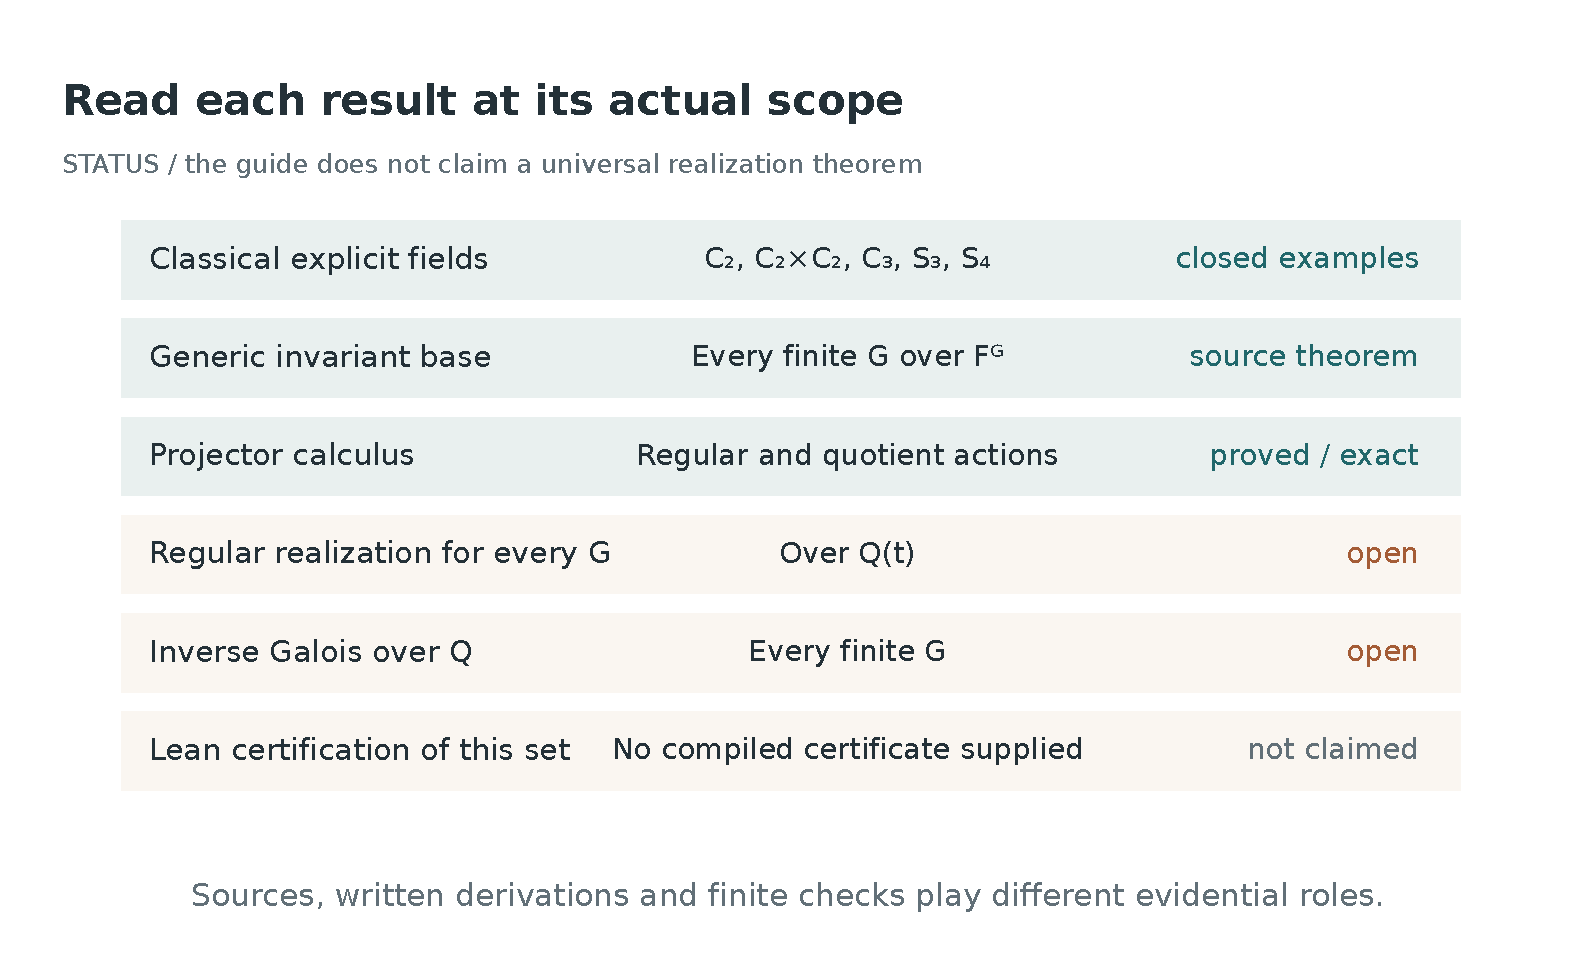
\includegraphics[width=0.94\linewidth]{../visual/figures/21_status_map.pdf}
\caption{Evidence has several roles. Written project arguments, external classical existence theorems, exact finite examples and the unresolved general realization question are recorded separately. The October 2026 preprint is attributed as dated context.}
\label{fig:g08-status}
\end{figure}

\section{Three precise routes to pursue}

An invariant-field route should begin with a specified action and a proposed rational parametrization. It must prove that the displayed invariants generate the fixed field, establish their algebraic relations and verify any claimed algebraic independence. A list of invariant polynomials or a correct transcendence-degree count does not identify the entire field. If a parametrization is obtained, the Hilbert step must retain the full extension and avoid the complete exceptional locus.

A cover route should begin with an actual finite Galois extension over $\Q(t)$. It must establish the group over that base and the absence of new algebraic constants. A construction over an algebraic closure does not itself prove descent to $\Q$. An ordinary number field with an added transcendental parameter does not automatically become a regular realization. The base, constant field and descent data must be visible in the statement.

An embedding-problem route should begin with a specified quotient and extension group. It must construct a continuous compatible lift and then prove surjectivity. In an exact sequence $1\to N\to E\to G\to1$, solving the equations in a small quotient model does not establish that the absolute Galois group has a proper solution. Conversely, failure in the finite $C_2$ toy is not a counterexample for the absolute Galois group. The ambient profinite domain is part of the arithmetic problem.

The certificate route is an additional way to organize a completed construction. It can guide local checking even when the field is discovered by one of the other routes. The theorem does not replace the difficult task of obtaining an irreducible degree-$|G|$ field presentation together with the compatible automorphisms.

\begin{openproblem}
For a stated class of finite groups beyond the externally known sectors used here, provide one complete arithmetic realization route. Specify its field or cover, rational base, full group certificate and any external theorem inputs. Every asserted uniform family needs a proof for all groups in that family.
\end{openproblem}

\section{The role of the resolution language}

The Galois part of Resolution Theory gives a coherent way to keep named fixed objects, mixed corners, subgroup refinements and normal quotients together. It makes information loss visible: a nonregular representation can erase a subgroup average, and a linear coordinate change does not by itself remember multiplication. It also gives an explicit location for the arithmetic input: the realization of the field and its base.

That is the contribution evaluated in this piece. The results are rooted in classical Galois and representation theory, with the project organizing their preservation and their failure modes in a common language. The reader does not claim that a renamed projector is a new existence theorem. Its stronger conclusions are the exact statements already proved under their hypotheses. Its research questions retain the missing hypotheses rather than concealing them in the word realization.

\begin{figure}[tbp]
\centering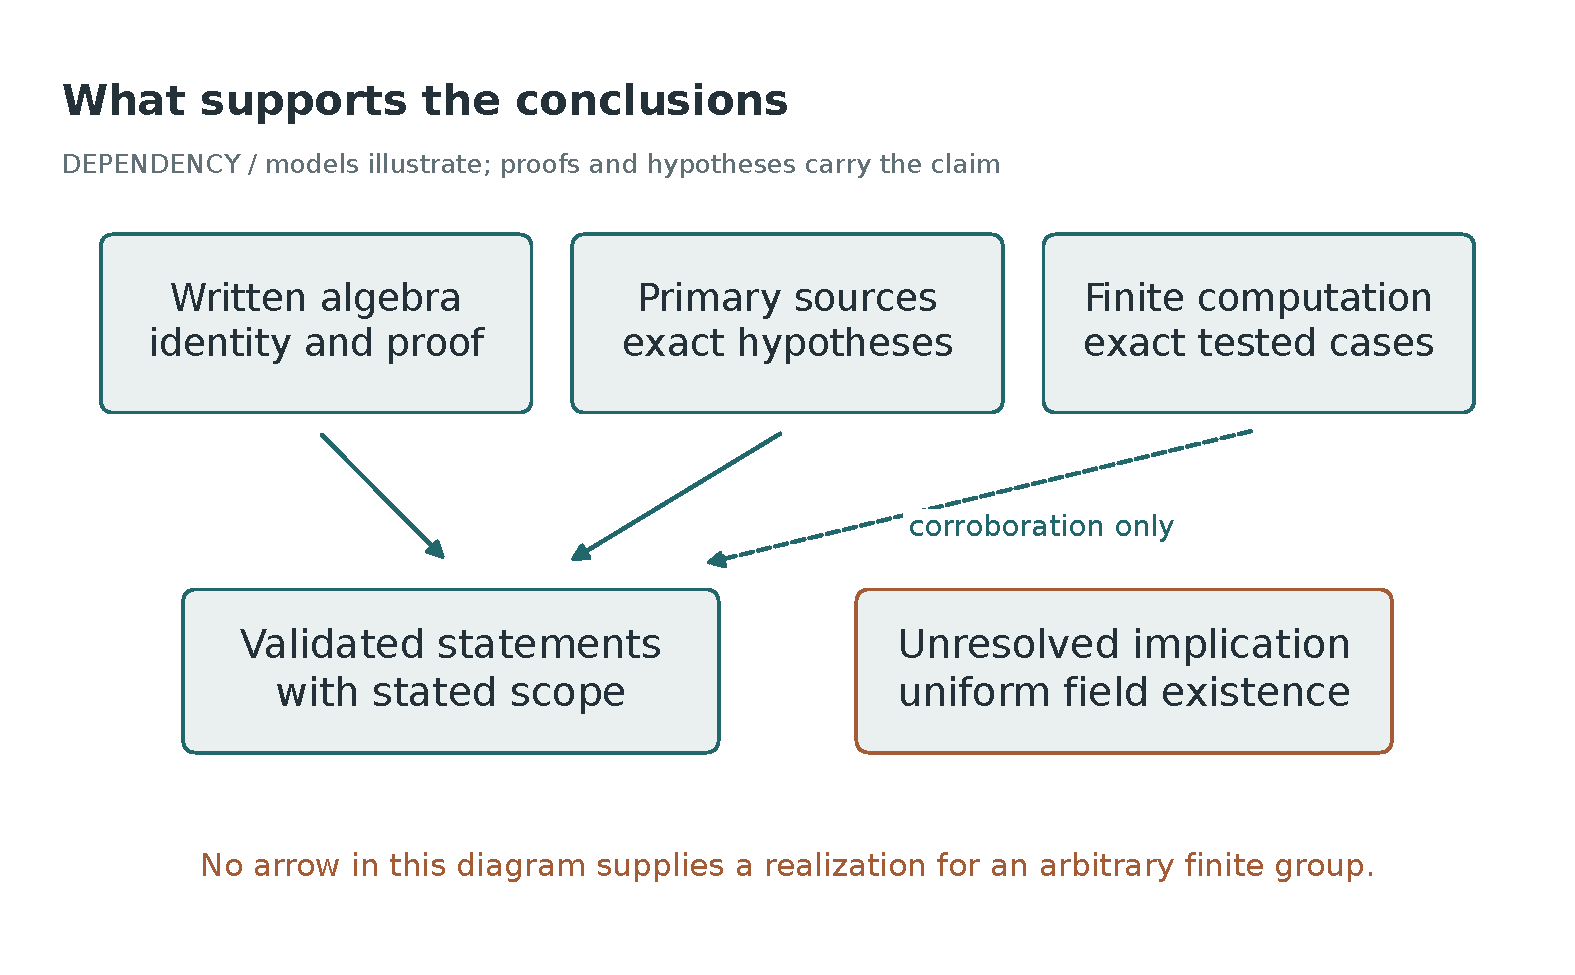
\includegraphics[width=0.94\linewidth]{../visual/figures/22_dependency.pdf}
\caption{A completed arithmetic conclusion requires an actual field and a full group argument. The generic invariant-field route and the regular-cover route reach that conclusion through their stated additional inputs. Finite matrix checks support examples and do not replace those inputs.}
\label{fig:g08-dependency}
\end{figure}


\appendix
\chapter{Conventions, source contracts and exact runs}
\label{app:g09-evidence}

\section{Notation and coefficient domains}

The symbol $G$ denotes a prescribed finite group, except where explicitly identified with the full Galois group of an existing extension. The arithmetic base is $\Q$. The field $E=\Q(x_g:g\in G)$ in Chapter~\ref{chap:g03-generic} is also written $F$ in the visual plates. Its invariant field is $K=E^G$. The equality $[E:K]=|G|$ describes a finite extension over $K$, while $E/\Q$ has positive transcendence degree.

The group-algebra arguments use the left regular module over $\C$, with a rational matrix model in the finite examples. If $\lambda(g)e_x=e_{gx}$, the orbits of the left $H$ action are the right cosets $Hx$. The normalized average is $E_H=|H|^{-1}\sum_{h\in H}\lambda(h)$. In the field-action formulation the same averaging operator is sometimes denoted $P_H$. A normal basis identifies the modules only after a finite Galois field has been supplied.

Subgroup inclusion reverses fixed-field inclusion. In the regular module, $H\subseteq K$ gives $\operatorname{ran}(E_K)\subseteq\operatorname{ran}(E_H)$. Commuting subgroup averages correspond to permutable products $HK=KH$ in the regular representation. Group faithfulness alone does not justify the converse. The exact $S_4$ example in Chapter~4 demonstrates the difference.

An arithmetic embedding problem uses the profinite group $G_{\Q}=\Gal(\overline{\Q}/\Q)$ with its Krull topology. A finite target group has the discrete topology. The lift is continuous, compatible with the prescribed quotient, and proper when surjective. The finite cyclic examples in Chapter~6 use a different ambient group and are explicitly models.

\section{External inputs retained by the proof chain}

\begin{longtable}{@{}p{.12\linewidth}p{.79\linewidth}@{}}
\toprule Contract & Exact input and scope\\\midrule\endhead
LC03 & Hilbert specialization over $\Q$, with the full primitive extension and nonzero exceptional-locus restrictions. One parameter and several parameters have different excluded sets.\\[4pt]
LC04 & Every finite solvable group occurs over $\Q$, from the corrected Shafarevich proof source. Additional local prescriptions are outside this statement.\\[4pt]
LC08 & Good-prime squarefree factor degrees yield a cycle in the characteristic-zero splitting-field group of a monic integral polynomial.\\[4pt]
LC09 & Irreducible cubic discriminant classification over $\Q$. The characteristic restrictions in the source are recorded explicitly.\\[4pt]
LC10 & Artin's finite automorphism theorem for an actual field with faithful finite automorphism group.\\[4pt]
LC11 & The subgroup/fixed-field correspondence for an extension already known to be finite Galois.\\[4pt]
LC12 & Normal basis for a finite Galois extension. This is a vector-space identification, not a field construction.\\[4pt]
LC13 & Trace and norm formulas and tower composition for the separable extensions used here.\\[4pt]
LC14 & Versioned $M_{23}$ preprint context, outside the elementary proof dependencies and not independently computationally reproduced.\\[4pt]
LC15 & Noether rationality as a sufficient conditional route. Contextual negative examples are source-attributed rather than independently audited here.\\[4pt]
LC16 & Continuous finite quotients of the absolute Galois group correspond to finite Galois field extensions.\\[4pt]
LC17 & Every existing finite separable extension has a primitive element, so a completed characteristic-zero realization admits the certificate format.\\
\bottomrule
\end{longtable}

The full contracts include exact source versions, printed page numbers, notation translations and acquisition diagnostics. They are under \texttt{literature/} in the source bundle. The bibliography records primary source URLs. Full third-party copies are omitted from the distributed bundle.

\section{The finite computation actually executed}

The script \texttt{computations/exact\_examples.py} uses exact rational, permutation and finite-field arithmetic. It records five scalar polynomials and their discriminants. It verifies the quartic's reductions at two and seven. It constructs all six subgroups of $S_3$ and checks all $36$ ordered pairs, including each subgroup paired with itself. It also records the faithful standard $S_4$ representation example, two finite lifting models and the three specialization values zero, one and two.

For the ordered basis
\[
 (),\ (23),\ (12),\ (123),\ (132),\ (13)
\]
the script constructs matrix columns from $\lambda(g)e_x=e_{gx}$. Every entry is an exact rational number. The $H=\langle(12)\rangle$ and $K=\langle(23)\rangle$ commutator is nonzero. Matrix ranks are computed over $\Q$, not with a floating tolerance. The figure source reads the frozen JSON generated by the same run. The individual roots plotted in the complex plane are numerical illustrations, not group certificates.

The bounded execution wrapper records the actual command, software versions, input hashes before and after execution, runtime, resource limits and output hashes in a version~2 manifest. Its validator passed with the project root supplied. An independent reviewer reconstructed the subgroup matrices from coset incidence and enumerated the subsets of $S_3$ to check that the stated six-subgroup range is complete. These checks support the finite records. The universal projector theorem still uses its written argument.

\section{Reproduction}

From the extracted bundle root, the portable exact calculation is
\begin{lstlisting}
python3 computations/exact_examples.py \
  --output computations/exact_examples.json
\end{lstlisting}
Python and SymPy are required. The bounded provenance wrapper additionally requires a POSIX environment for its enforced limits:
\begin{lstlisting}
python3 computations/run_examples.py
\end{lstlisting}
That wrapper creates the evidence logs, manifest and scientific JSON, then copies the same JSON bytes to the figure input path. It does not depend on a random seed. The shipped manifest records the versions actually used, rather than guaranteeing byte-identical serialized output for all future library versions.

Rebuild the readers with
\begin{lstlisting}
python3 build.py --figures
\end{lstlisting}
The PDF and scientific plotting dependencies are listed in the bundle README. Rebuilding can change PDF hashes or page flow. The delivered page-review records apply to the delivered PDFs, and a changed build needs renewed visual inspection. Compilation alone is not a layout review or a mathematical proof.

The four original recovered inputs are retained in \texttt{historical/}. Their byte counts and hashes are checked separately. Historical audits retain their original scope. The current manuscript, exact calculations, source contracts, proof review and page reviews supply this edition's claim boundary.

\backmatter
\renewcommand{\bibname}{Primary sources}
\begin{thebibliography}{9}
\addcontentsline{toc}{chapter}{Primary sources}

\bibitem{Milne2022}
J. S. Milne.
\emph{Fields and Galois Theory}.
Kea Books, 2022.
Author-hosted edition, checked 9 October 2026.
\url{https://www.jmilne.org/math/Books/FT0.pdf}.

\bibitem{SchmidtWingberg1998}
Alexander Schmidt and Kay Wingberg.
\emph{Safarevi\v{c}'s theorem on solvable groups as Galois groups}.
\texttt{arXiv:math/9809211v1}, 17 September 1998.
Theorem 1 gives the corrected solvable realization input.
\url{https://arxiv.org/abs/math/9809211v1}.

\bibitem{DebesHarbater2021}
Pierre D\`ebes and David Harbater.
Pre-Galois theory.
\emph{Osaka Journal of Mathematics} \textbf{58} (2021), 71--101.
Published author-hosted copy.
\url{https://pro.univ-lille.fr/fileadmin/user_upload/pages_pros/pierre_debes/A59-DebesHarbater2.pdf}.

\bibitem{DebesLectureNotes}
Pierre D\`ebes.
\emph{Arithm\'etique des rev\^etements de la droite}.
Author lecture manuscript, 385-page snapshot checked 9 October 2026.
The author publication page describes a 2024 work in progress.
Theorems 2.6.3 and 5.2.4 and Proposition 5.2.14 supply the specialization input.
\url{https://pro.univ-lille.fr/fileadmin/user_upload/pages_pros/pierre_debes/V2-ArithRevDte-v3.pdf.pdf}.

\bibitem{Debes2026}
Pierre D\`ebes.
\emph{Hurwitz spaces and inverse Galois theory}.
Author manuscript dated 9 April 2026, 27 pages.
\url{https://pro.univ-lille.fr/fileadmin/user_upload/pages_pros/pierre_debes/A67-Nakamura60.pdf}.

\bibitem{HuangEtAl2026}
Xiaoyu Huang, Blake Jackson, Kyu-Hwan Lee, Bjorn Poonen,
Rachel Pries and Shaowu Zhang.
\emph{The Mathieu group $M_{23}$ is a Galois group over $\mathbb Q$}.
\texttt{arXiv:2608.08538v2}, submitted 7 October 2026.
Manuscript dated 4 October 2026. Preprint used for dated context.
\url{https://arxiv.org/abs/2608.08538v2}.

\bibitem{ConradCyclotomic}
Keith Conrad.
\emph{Cyclotomic Extensions}.
Undated author notes, snapshot checked 9 October 2026.
\url{https://kconrad.math.uconn.edu/blurbs/galoistheory/cyclotomic.pdf}.

\bibitem{ConradPatternsPrimes}
Keith Conrad.
\emph{Patterns in Primes}.
Undated author notes, snapshot checked 9 October 2026.
Theorem 2.4 states the classical Dirichlet input.
\url{https://kconrad.math.uconn.edu/blurbs/ugradnumthy/prime-patterns-1.pdf}.

\end{thebibliography}

\end{document}
